\documentclass[a4paper]{book}
\usepackage{graphicx}
\usepackage[breaklinks=true]{hyperref}
\usepackage{listings}
\usepackage{color}
\usepackage{makeidx}
\usepackage{rotating}
\usepackage{tocbibind}
\usepackage{fancyhdr}
\usepackage{natbib}
\usepackage{chemformula}
\usepackage{siunitx}
\usepackage{caption}

\usepackage{tikz}
\usetikzlibrary{arrows,shapes.geometric,positioning,graphs,calc}
\usepackage{tikz-3dplot}
\usepackage[outline]{contour} % glow around text
\usepackage{xcolor}
\tikzstyle{plane}=[black!80,line width=0.08] %very thin
\contourlength{1.3pt}

\renewcommand{\familydefault}{\sfdefault}

\lstset{
breakatwhitespace=true,
language=tcl,
columns=fullflexible,
keepspaces=true,
breaklines=true,
tabsize=3, 
showstringspaces=true,
extendedchars=true,
  basicstyle=\small\ttfamily,
  frame=lrtb,
  numbers=left,
  keywordstyle=\color{blue}
}

% Add mmonca keywords here
\lstset{emph={%  
    anneal, cascade, extract, init, insert, lowmsg, param, profile, report, save, test%
    },emphstyle={\color{red}\small\ttfamily}%
}%

\pagestyle{fancy}
\fancyhf{}
\fancyhead[RO]{
\includegraphics[width=1cm]{images/logo} user guide}
\fancyhead[LE]{
\includegraphics[width=4mm]{images/AMM}\leftmark}
\fancyfoot[LE,RO]{\thepage}

\newcommand{\specialcell}[2][c]{%
  \begin{tabular}[#1]{@{}c@{}}#2\end{tabular}}

\newcommand{\param}[1]{{\tt #1}\index{#1}}
\newcommand{\idx}[1]{#1\index{#1}}
\newcommand{\MMonCa}{
\includegraphics[width=1cm]{images/logo}}

\renewcommand{\cite}{\citet}

\makeindex

\author{Originally develop at the IMDEA Materials Institute\\
Currently supported at github.com/imartinbragado/MMonCa}

\title{
\includegraphics[width=12cm]{images/logo}}

\begin{document}
\maketitle
\tableofcontents


\newpage
\chapter{Preliminaries}

\section{Citing}

Please, if using \MMonCa\ cite it as in Ref.~\cite{MARTIN-BRAGADO-CPC13}.
If you use the LKMC module only, you can cite Ref.~\cite{MARTIN-BRAGADO-APL11}.
If using the BCA software (Ion Implant Simulator) cite
Ref.~\cite{HERNANDEZ-MANGAS-JAP02}


\section{Introduction}
\subsection{Installation from source code}
\begin{enumerate}
 \item Download and unpack the \MMonCa\ source code from the IMDEA Materials web page. {\tt http://www.materials.imdea.org/MMonCa}.
 \item Be sure you have a modern version of the {\tt g++} compiler installed in your system. 
\begin{itemize}
\item Type \param{make} to obtain some help on how the \param{Makefile} system works.
\item The make command expects one \param{machine} to be specified. The available machines are in the directory \param{sysmakes}.
\item Each \param{machine} is a specific configuration for a particular architecture. The \param{make} commands creates a binary directory called {\tt Obj\verb+_+machine} directory, with the \param{mmonca} binary inside.
\end{itemize}
\item The compilation system looks for several libraries. Some of them are compulsory, other optional if you want to have the \param{iris} FEM module running. In an Ubuntu or Debian system these libraries can be installed using \param{apt-get}. The required libraries (for Ubuntu) are:
\begin{description}
\item[compulsory] {\tt tcl-dev}.
\item[compulsory] {\tt libboost-dev}.
\item[compulsory] {\tt libboost-iostreams-dev}
\item[iris] {\tt libsuperlu3-dev}.
\item[iris] {\tt liblapack-dev}.
\end{description}
 \item Depending on the location of your workspace, add the following line to {\tt .bashrc: export MCPATH=/home/\textit{username}/workspace/MMonCa/config}
 \item After compiling the code navigate to ({\tt cd} command): \\
{\tt /home/\textit{username}/workspace/MMonCa/test}, and enter {\tt runAll.sh} in order to run the KMC tests and confirm a successful installation. The test suite expects a MMonCa binary in a directory called Release. You can copy or link a binary there for the test suite to work. By default, it uses the binary inside \verb-Obj_g++-.
\end{enumerate}



\subsection{Submission Policy}
\index{submission}
When collaborating on a program, it is essential to preserve the functionality of existing code before adding your own. Therefore, after code is developed it is important to run all existing \param{test} to check that there are no failures. Also, new tests are required to be created for every new feature in the code.

The test-suite can be run with the command \param{runAll.sh} in the \param{test} directory as previously explained.

\subsection{Installation from binary sources}
\begin{itemize}
\item Untar and unzip the \MMonCa\ binary with something like:
\begin{verbatim}
tar -xvzf MMonCa-VERSION-bin.tar.gz
\end{verbatim}
\item Be sure you have the following libraries installed in your system:
\begin{itemize}
\item libtcl
\item libblas
\item liblapack
\item libsuperlu
\end{itemize}
 \item Depending on the location of your workspace, add the following line to {\tt .bashrc: export MCPATH=/home/\textit{username}/workspace/MMonCa/config}.\index{MCPATH}
\end{itemize}

\section{Mechanical settings}
\index{Mechanics}

There are three different modules to produce mechanical output (strain and stress) for \MMonCa. These modules can be set up with the command:

\begin{lstlisting}
param set type=string key=Mechanics/General/model  value=module
\end{lstlisting}

The different available modules are:
\begin{description}
\item[\param{Feliks}] Realistic calculation of stresses and strains by calling the finite element solver included in \MMonCa\ and developed by
\idx{Ignacio} Romero at the Technical University.
\item[\param{Uniform}] Simple model that allows to specify a fixed value in \param{Mechanics/Uniform}. The values are \param{stress.xx}, \param{stress.yy} and \param{stress.zz}.
\item[\param{None}] No model.
\end{description}

\subsection{Testing MMonCa}

\MMonCa\ includes a test suite of several test cases. If you want to check the integrity of the distribution, or whether yuor compilation is correct, all tests should be run and should pass. Sometimes few tests might fail even when the distribution is correct if it was compiled in an architecture different than the original. The original architecture is \param{Ubuntu} LTS 14.04. In this cases, the failing cases are usually a little bit out of the random variation allowed in the original architecture. 

All the tests are in the \param{test} subdirectory. The following scripts are available:

\begin{description}
\item [\param{runAll.sh}] To run all the tests and display the results.
\item [\param{runFailed.sh}] To run only the failing tests and display all the results.
\item [\param{collect.sh}] To display the results only, no running of tests.
\end{description}


\chapter{Running MMonCa}

\section{Generalities}

To run a \MMonCa\ script just call the {\param mmonca} binary with the input file you want to execute as a parameter name.

\begin{lstlisting}
mmonca input.mc
\end{lstlisting}

The input scripts are regular \param{TCL} scripts that include additional MMonCa commands. All regular TCL commands (to manipulate variables, loops, procedures, etc) should be available. For a list of the additional commands included in \MMonCa\ allowing Monte Carlo simulations and post-processing of information, consult Chapter~\ref{chap:commands}.

\subsection{Starting from scratch}

The following is a list of required and optional instructions that should be provided in a \MMonCa\ script when starting from scracth:

\begin{description}
\item [required] Telling MMonCa with materials to use by setting {\param MC/General/materials}
\item [required] Defining the distribution of materials in space with a procedure ({\tt proc material} in this case)
\item [optional] Redefining some extra parameters with \param{param}.
\item [required] Initializing the simulation box with \param{init}.
\item [optional] Reading the initial damage to anneal with \param{cascade}.
\item [required] Letting the system evolve in time with the \param{anneal}.
\item [optional] Obtaining some useful information with \param{extract}.
\item [optional] Saving some information for visualization purposes with \param{save}.
\item [optional] Saving the simulation status for restarting with \param{restart}.
\end{description}

\subsection{Restarting}

An alternative is to start \MMonCa\ from a file saved with the \param{restart} option. In this case, the following is the list of required and optional instructions:
\begin{description}
\item [required] Using the \param{restart} option as the first command.
\item [optional] Redefining some extra parameters with \param{param}.
\item [optional] Reading the initial damage to anneal with \param{cascade}.
\item [optional] Letting the system evolve in time with the \param{anneal}.
\item [optional] Obtaining some useful information with \param{extract}.
\item [optional] Saving some information for visualization purposes with \param{save}.
\item [optional] Saving the simulation status for further restarting with \param{restart}.
\end{description}


\section{Object Kinetic Monte Carlo simulation: an example}

The following is an example of a \MMonCa\ input script, taken from Ref.~\cite{MARTIN-BRAGADO-CPC13}, that performs the isochronal annealing of $\alpha$-Fe. The goal is to simulate the evolution of defects and resistivity recovery during isochronal annealing of high-purity electron-irradiated iron. The script contains both the commands needed to set the simulation conditions, and the commands required to do some post-processing of information, mainly extracting the evolution of defects with time to an external file. There are also typical \param{TCL} commands that help in the extraction. 

The initial damage in this example is read from an {\tt electron.cascade} file containing the IV pairs produced by electron irradiation.

This example can be found in the {\param examples} directory.

\subsection{The script}

\begin{lstlisting}
param set type=map<string,string>   key=MC/General/materials value="S_Iron Fe"
set size 143.5
set time 300

proc material { x y z } { return "S_Iron" }

#parameters
param set type=bool   key=MC/Mesh/periodic.x value=true

param set type=arrhenius key=S_Iron/Vacancy/V(migration)   value="5e-5 0.67"
param set type=arrhenius key=S_Iron/Iron/I(migration)      value="3.2e-3 0.34"

init minx=0 miny=0 minz=0 maxx=$size maxy=$size maxz=$size material=material

cascade file=electron.cascade format=B:C*.287:D*.287:E*.287 periodic flux=4.8562e9 do.not.react

set X 0
set a 77.2
set b 1.030927

set FILE [open "results.txt" w]
close $FILE

set oldTotal 0
set oldC 0

save ovito=evolution
while { $X < 65 } {
      incr X
      set c [expr $a*$b]
      lowmsg "Running for $c K"      
      set FILE [open "results.txt" a]
      anneal time=$time temp=[expr $c - 273.15]
      save ovito=evolution append
      set total [extract count.particles]
      set deriv [expr ($total - $oldTotal)/($c - $oldC)]
      set I     [extract count.particles particle=I defect=MobileParticle]
      set V     [extract count.particles particle=V defect=MobileParticle]
      set I2    [extract count.particles defect=ICluster ID=I2]
      set V2    [extract count.particles defect=VCluster ID=V2]
      set I3    [extract count.particles defect=ICluster ID=I3]
      set V3    [extract count.particles defect=VCluster ID=V3]
      set I111  [extract count.particles defect=<111>]
      set oI    [expr [extract count.particles defect=ICluster] -$I2 -$I3]
      set oV    [expr [extract count.particles defect=VCluster] -$V2 -$V3]
      puts $FILE "$c $total $deriv $I $V $I2 $V2 $I3 $V3 $oI $oV $I111"
      lowmsg     "$c $total $deriv $I $V $I2 $V2 $I3 $V3 $oI $oV $I111"
      close $FILE
      set a $c
      set oldC $c
      set oldTotal $total
}
\end{lstlisting}

\subsection{The script, dissected}

\begin{lstlisting}
param set type=map<string,string>   key=MC/General/materials value="S_Iron Fe"
\end{lstlisting}
Line needed to define the materials to be used in the simulation.

\begin{lstlisting}[firstnumber=2]
set size 143.5
set time 300
\end{lstlisting}
TCL variables defined to easily change the simulation size and the annealing times between steps.

\begin{lstlisting}[firstnumber=5]
proc material { x y z } { return "S_Iron" }
\end{lstlisting}
Required script to define the material in the simulation. In this case, a block containing only Iron is defined.

\begin{lstlisting}[firstnumber=7]
#parameters
param set type=bool   key=MC/Mesh/periodic.x value=true
param set type=arrhenius key=S_Iron/Vacancy/V(migration)   value="5e-5 0.67"
param set type=arrhenius key=S_Iron/Iron/I(migration)      value="3.2e-3 0.34"
\end{lstlisting}
Some redefinition of parameters: setting of periodic boundary conditions in x (false by default, because there are usually free surfaces in this axis), and small changes in point defect migration parameters.

\begin{lstlisting}[firstnumber=13]
init minx=0 miny=0 minz=0 maxx=$size maxy=$size maxz=$size material=material
\end{lstlisting}
Required initialization of the simulator, specifying the simulation sizes and the script containing the material definition. In this case, we are using the TCL variables, previously defined, {\tt size}.

\begin{lstlisting}[firstnumber=15]
cascade file=electron.cascade format=B:C*.287:D*.287:E*.287 periodic flux=4.8562e9 do.not.react
\end{lstlisting}
Initial conditions for the simulation: insertion of damage. This command is not strictly needed, but is very common, because damage has to be introduced to simulate its evolution, unless equilibrium concentrations want to be set.

\begin{lstlisting}[firstnumber=17]
set X 0
set a 77.2
set b 1.030927
\end{lstlisting}
Definition of some convenient TCL variables to later compute the temperature ramps.

\begin{lstlisting}[firstnumber=21]
set FILE [open "results.txt" w]
close $FILE
\end{lstlisting}
This confusing commands open a file to close it right away. The goal is to overwrite previous existing files with an empty file. Later, information will be appended to the file.

\begin{lstlisting}[firstnumber=24]
set oldTotal 0
set oldC 0
\end{lstlisting}
Definition of TCL variables to compute the first derivative of the total damage.

\begin{lstlisting}[firstnumber=27]
save lammps=evolution
\end{lstlisting}
Command to create a initial file with the atomistic information, using the \param{lammps} format that can be later used by \param{ovito} to visualize the information. More save commands will be issued later to \param{append} new time frames into the file.

\begin{lstlisting}[firstnumber=28]
while { $X < 65 } {
      incr X
      set c [expr $a*$b]
      lowmsg "Running for $c K"      
\end{lstlisting}
Initialization of the loop to increase the temperature, and operations to compute the next temperature for the annealing.

\begin{lstlisting}[firstnumber=32]
      set FILE [open "results.txt" a]
\end{lstlisting}
TCL command to open an (existing) file and append information to it.

\begin{lstlisting}[firstnumber=33]
      anneal time=$time temp=[expr $c - 273.15]
\end{lstlisting}
The fundamental \param{anneal} command, needed to start the annealing of defects in time. Both the time and temperature need to be specified, in this case, using TCL variables defined previously. Since the temperature in ``c'' is in Kelvin, but the anneal command requires the temperature to be written in Celsius, a translation is defined in line.

\begin{lstlisting}[firstnumber=34]
      save lammps=evolution append
\end{lstlisting}
Command to append one more snapshot for visualization

\begin{lstlisting}[firstnumber=35]
      set total [extract count.particles]
      set deriv [expr ($total - $oldTotal)/($c - $oldC)]
      set I     [extract count.particles particle=I defect=MobileParticle]
      set V     [extract count.particles particle=V defect=MobileParticle]
      set I2    [extract count.particles defect=ICluster ID=I2]
      set V2    [extract count.particles defect=VCluster ID=V2]
      set I3    [extract count.particles defect=ICluster ID=I3]
      set V3    [extract count.particles defect=VCluster ID=V3]
      set I111  [extract count.particles defect=<111>]
      set oI    [expr [extract count.particles defect=ICluster] -$I2 -$I3]
      set oV    [expr [extract count.particles defect=VCluster] -$V2 -$V3]
      puts $FILE "$c $total $deriv $I $V $I2 $V2 $I3 $V3 $oI $oV $I111"
      lowmsg     "$c $total $deriv $I $V $I2 $V2 $I3 $V3 $oI $oV $I111"
      close $FILE
\end{lstlisting}
Post-processing of the information after each annealing. The number of particles for different defect types is asked, and stored in TCL variables.  These variables are used to add one line to the previously opened file, with the different values, then allowing to have a file with different columns, and the number of particles of different defects in each column. The derivative of the number of defects is also computed.

\begin{lstlisting}[firstnumber=49]
      set a $c
      set oldC $c
      set oldTotal $total
}
\end{lstlisting}
Variable operations to update the temperature ramp, and to make possible the computation of the first derivative. End of the script.

\subsection{The output}

The script creates a list named {\tt results.txt} that looks like:
\begin{verbatim}
79.58756439999999 59955 753.3212060450993 29962 29993 0 0 0 0 0 0 0
82.04896900419878 59955 0.0 29962 29993 0 0 0 0 0 0 0
84.58649746859163 59953 -0.7881684986255068 29961 29992 0 0 0 0 0 0 0
87.20250407580276 59937 -6.116192503449846 29953 29984 0 0 0 0 0 0 0
89.8994159193551 59917 -7.415889417303392 29943 29974 0 0 0 0 0 0 0
92.67973515549299 59813 -37.40577651955731 29891 29922 0 0 0 0 0 0 0
95.54604132464692 59453 -125.59718981669849 29711 29742 0 0 0 0 0 0 0
98.50099374469427 58089 -461.5979569573388 29029 29060 0 0 0 0 0 0 0
101.54733397823642 54015 -1337.342413412217 26978 27023 14 0 0 0 0 0 0
104.68788837618133 43219 -3437.6096166538605 21560 21625 34 0 0 0 0 0 0
107.92557069999148 23693 -6030.857276022542 11749 11862 82 0 0 0 0 0 0
111.26338482503012 9445 -4268.661904543617 4601 4738 106 0 0 0 0 0 0
114.70442752751381 6359 -896.8211867212708 3060 3195 104 0 0 0 0 0 0
118.25189135765723 5303 -297.6774536859221 2516 2667 120 0 0 0 0 0 0
121.90906760167549 4757 -149.2955120478667 2229 2394 134 0 0 0 0 0 0
125.6793493353925 4399 -94.95311631448243 2015 2215 166 0 3 0 0 0 0
129.56623457228818 4087 -80.26992848628163 1811 2059 214 0 3 0 0 0 0
133.57332950890532 3801 -71.3734025581751 1493 1916 374 0 18 0 0 0 0
137.70435187062722 3439 -87.62963942153782 1100 1735 500 0 96 0 8 0 0
141.9631343609301 2967 -110.82979726593929 611 1499 604 0 213 0 40 0 0
146.3536282173106 2535 -98.39439801793499 229 1283 604 0 303 0 108 0 8
150.87990687718735 2327 -45.9538653339702 44 1179 578 0 327 0 184 0 15
\end{verbatim}

\begin{figure}
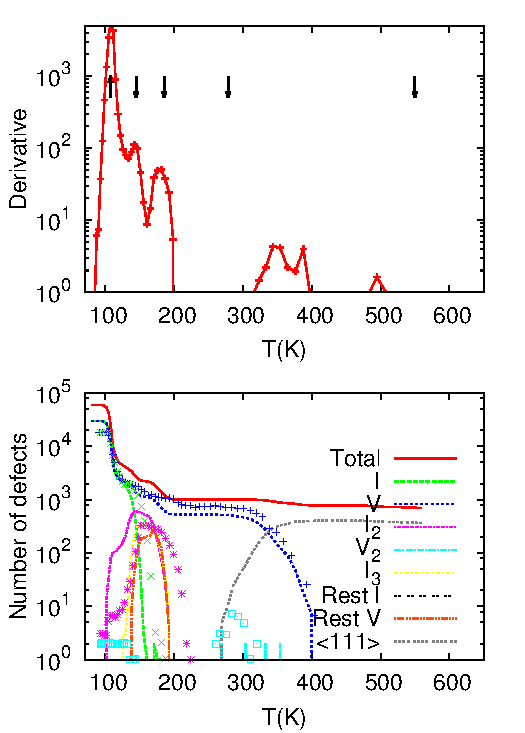
\includegraphics{images/Fe}
\caption{Isochronal annealing of Iron. \cite{MARTIN-BRAGADO-CPC13}}
\label{fig:isochronalFe}
\end{figure}


Fig.~\ref{fig:isochronalFe} shows the results processed with the \param{gnuplot} tool.



\section{Lattice Kinetic Monte Carlo simulation: an example}

In this section we will show an input script that, using the Lattice Kinetic Monte Carlo model, simulates the Si(100), Si(011) and Si(111) Solid Phase epitaxial regrowth of a partially amorphized sample, and computes its recrystallization speed and roughness. These scripts used the models published in Refs.~\cite{MARTIN-BRAGADO-APL09,MARTIN-BRAGADO-APL11,MARTIN-BRAGADO-SM12,MARTIN-BRAGADO-JAP12}, and are partially based in the scripts distributed under the folder \param{tests}, sub-folders {\tt standard/lkmc}.

\subsection{The script}

\begin{lstlisting}
param set type=map<string,string>   key=MC/General/materials value="Silicon Si AmorphousSilicon aSi Gas Gas"

set T 550
set name SPER
#0 9 or 14
set i 0
proc material { x y z } {
        set res "Unknown"
        if { $x < 0 } {
                set res "Gas"
        } elseif { $x < 52 } {
                set res "AmorphousSilicon"
        } else {
                set res "Silicon"
        }
        return $res
}

set angle(0)  00
set angle(9)  55
set angle(14) 90

set sizeZ    [expr sqrt(2.)*.5431*26]
set sizeY    [expr 180]

param set type=bool key=MC/Mesh/periodic.y value=false
param set type=bool key=MC/Mesh/periodic.z value=true

set radians "$angle($i).0*2.0*3.1415926535897931/360.0"
set S [expr sin($radians)]
set C [expr cos($radians)]
set R [expr sqrt(2.0)]
set waferorient "i $C  j [expr $S/$R] k [expr $S/$R]"
set flatorient  "i -$S j [expr $C/$R] k [expr $C/$R]"

param set type=map<string,float> key=Silicon/Lattice/wafer.orientation value="$waferorient"
param set type=map<string,float> key=Silicon/Lattice/flat.orientation  value="$flatorient" 
param set type=map<string,float> key=AmorphousSilicon/Lattice/wafer.orientation value="$waferorient"
param set type=map<string,float> key=AmorphousSilicon/Lattice/flat.orientation  value="$flatorient" 

init minx=-2 miny=0 minz=0 maxx=54 maxy=$sizeY maxz=$sizeZ material=material

anneal time=1 temp=$T depth=51
set orig_time [extract time]  
set orig_depth [lindex [extract ac.mean min.y=60 max.y=120 min.z=0 max.z=$sizeZ] 0]
lowmsg "Original depth is $orig_depth"

anneal time=1 temp=$T depth=31
set end_time [extract time]   
set end_depth [lindex [extract ac.mean min.y=60 max.y=120 min.z=0 max.z=$sizeZ] 0]
lowmsg "$angle($i) - Final depth is $end_depth"
set velocity [expr ($orig_depth - $end_depth)/($end_time-$orig_time)*60]
set roughnes [extract ac.stdev]
lowmsg "Velocity  for angle $angle($i) is $velocity in nm/min."
lowmsg "Roughness for angle $angle($i) is $roughnes in nm."

\end{lstlisting}

\subsection{The script, dissected}

This script adds the complication that it has been done to accept different substrate orientation with minimum changes in the script. This complication is managed using a TCL array called {\tt angle}, and used to compute the substrate orientation automatically. Also, since having periodic boundary conditions is not possible for all possible substrate orientations, the script defines a quite large $y$ domain (180\,nm) without boundary conditions, but measures the recrystallization velocity only in the middle of the domain, where it is expected to be flat.

\begin{lstlisting}
param set type=map<string,string>   key=MC/General/materials value="Silicon Si AmorphousSilicon aSi Gas Gas"
\end{lstlisting}
Definition of the materials used.

\begin{lstlisting}[firstnumber=3]
set T 550
set name SPER
\end{lstlisting}
Definition of temperature and script name, to be used later

\begin{lstlisting}[firstnumber=5]
#0 9 or 14
set i 0
\end{lstlisting}
The substrate angle is codified in this integer.

\begin{lstlisting}[firstnumber=7]
proc material { x y z } {
        if { $x < 0 } {
                set res "Gas"
        } elseif { $x < 52 } {
                set res "AmorphousSilicon"
        } else {
                set res "Silicon"
        }
        return $res
}
\end{lstlisting}
Definition of the materials. Three sections are defined, ``Gas'', for $x < 0$, ``AmorphousSilicon'' for $0 < x < 52$ and ``Silicon'' (i.e., crystalline silicon) for $x \geq 52$.

\begin{lstlisting}[firstnumber=19]
set angle(0)  00
set angle(9)  55
set angle(14) 90
\end{lstlisting}
Definition of an array indexed by integers with the possible angles. 0 for Si(100), 9 for Si(111) and 14 for Si(011). This infrastructure allows the definition of intermediate angles for the other $i$s.

\begin{lstlisting}[firstnumber=23]
set sizeZ    [expr sqrt(2.)*.5431*26]
set sizeY    [expr 180]
\end{lstlisting}
Definition of the size as a variable. $y$ should be big enough to have a flat region without periodic boundary conditions, but especial dimensions are set for $z$ to have periodicity.

\begin{lstlisting}[firstnumber=26]
param set type=bool key=MC/Mesh/periodic.y value=false
param set type=bool key=MC/Mesh/periodic.z value=true
\end{lstlisting}
Boundary conditions for $z$ only. By default $x$ has no PBC.

\begin{lstlisting}[firstnumber=29]
set radians "$angle($i).0*2.0*3.1415926535897931/360.0"
set S [expr sin($radians)]
set C [expr cos($radians)]
set R [expr sqrt(2.0)]
set waferorient "i $C  j [expr $S/$R] k [expr $S/$R]"
set flatorient  "i -$S j [expr $C/$R] k [expr $C/$R]"
\end{lstlisting}
Example of use of the TCL language embedded in the \MMonCa\ scripting to compute the substrate orientation.

\begin{lstlisting}[firstnumber=36]
param set type=map<string,float> key=Silicon/Lattice/wafer.orientation value="$waferorient"
param set type=map<string,float> key=Silicon/Lattice/flat.orientation  value="$flatorient" 
param set type=map<string,float> key=AmorphousSilicon/Lattice/wafer.orientation value="$waferorient"
param set type=map<string,float> key=AmorphousSilicon/Lattice/flat.orientation  value="$flatorient" 
\end{lstlisting}
Definition of the substrate orientation as a parameter, once computed previously.

\begin{lstlisting}[firstnumber=41]
init minx=-2 miny=0 minz=0 maxx=54 maxy=$sizeY maxz=$sizeZ material=material
\end{lstlisting}
Compulsory definition of the initial simulation box and initial materials.

\begin{lstlisting}[firstnumber=43]
anneal time=1 temp=$T depth=51
\end{lstlisting}
Since the amorphous/crystalline (A/C) interface is artificially flat plane (atomically flat) an small initial annealing (recrystallization) is issued to recrystallize a maximum of 1\,nm, creating an starting condition where the A/C interface is more realistic. 

\begin{lstlisting}[firstnumber=44]
set orig_time [extract time]  
set orig_depth [lindex [extract ac.mean min.y=60 max.y=120 min.z=0 max.z=$sizeZ] 0]
lowmsg "Original depth is $orig_depth"
\end{lstlisting}
Use of TCL to store the initial position of the interface.

\begin{lstlisting}[firstnumber=48]
anneal time=1 temp=$T depth=31
\end{lstlisting}
Main recrystallization: From depth 51 to depth 31, a maximum of 20\,nm is requested.

\begin{lstlisting}[firstnumber=49]
set end_time [extract time]   
set end_depth [lindex [extract ac.mean min.y=60 max.y=120 min.z=0 max.z=$sizeZ] 0]
lowmsg "$angle($i) - Final depth is $end_depth"
set velocity [expr ($orig_depth - $end_depth)/($end_time-$orig_time)*60]
set roughnes [extract ac.stdev]
\end{lstlisting}
The annealing command stops when the A/C touches the requested depth, but here we want to compute the recrystallization speed using average values, not maximum ones. Thus, the average depth is computed for $60 < y < 120$ and stored. The velocity is then computed using the regular $v=\frac{\Delta x}{\Delta t}$ equation. The roughness is extracted using a specific \MMonCa\ command.

\begin{lstlisting}[firstnumber=54]
lowmsg "Velocity  for angle $angle($i) is $velocity in nm/min."
lowmsg "Roughness for angle $angle($i) is $roughnes in nm."
\end{lstlisting}
Finally, the values are displayed.

\subsection{Simulation results}

Fig.~\ref{fig:lkmc-example} shows the results for Si(100), Si(011) and Si(111) simulations compared to experimental results taken from Ref.~\cite{CSEPREGI-JAP78}

\begin{figure}
\begin{center}
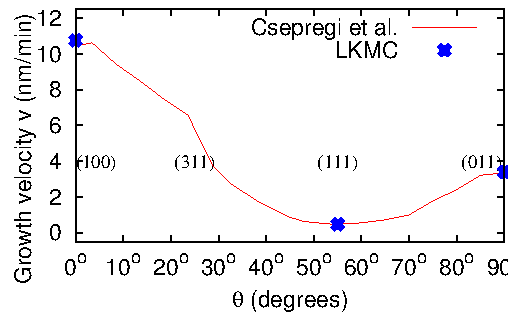
\includegraphics{images/csepregi}
\end{center}
\caption{Solid Phase Epitaxial Regrowth of amorphized silicon. \cite{MARTIN-BRAGADO-APL09}}
\label{fig:lkmc-example}
\end{figure}

\section{Parallelism}

\subsection{Standard}

``Poor man parallelization'' is implemented. It can be used with the parameter: \verb+/MC/General/domains+ set to the number of threads. Default is 1.

This type of \idx{parallelization} is done by simple splitting of the $z$ axis, as can be seen in Fig.~\ref{fig:poor-parallelization} and running in a totally independent way such splits in different threads, with no communication at all between them during the annealing. Insertion and extraction of information is, nevertheless, transparent to the user, meaning that the user input (cascade, profile, anneal) and output (extract) commands will work as if there is only 1 domain.

This parallelization is optimal when a better statistics is needed and there is 1D or 2D symmetry in the system. Special care has to be taken to be be sure that each domain is big enough to represent the physics of the system simulated. For example, if a system requires at least 20\,nm in the z axis, a simulation with at least $20\times n$, being $n$ the number of threads, needs to be run, because each thread will run a simulation with $20\times n / n = 20$\,nm in the z axis.

Parallel execution is also possible using the new nonuniform mesh. The simulation area is divided along the Z axis, but only at the division planes. This division happens possibly in a uniform way. Should the linesz resolution be too coarse somewhere, a domain may end up with 0 Z-size. This happens for example when one sets 16 domains but has only 6 division planes along the Z axis.. In this case, MMonCa exits with an error message.

Note, however, nonuniform meshes don't support more than 1 subdomains.

Alternative ways of parallelization are being currently studied. If you want to have more information ask {\tt ignacio.martin@imdea.org}.

\begin{figure}
\begin{center}
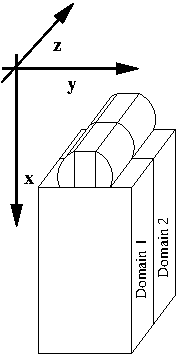
\includegraphics{images/poor-parallelization}
\end{center}
\caption{Simple parallelization splits the z domain in independent sub-domains and runs them isolated from each other. All input and output of information is transparent to the user.}
\label{fig:poor-parallelization}
\end{figure}

\subsection{Experimental}

Experimental parallelization based on the work of \cite{MARTINEZ-JCP08} has been implemented as explained in \cite{MARTIN-BRAGADO-NIMB15}. As explained in the cited paper, this parallelization works but should be used with extreme caution to avoid very slow simulations.


\chapter{Syntax}
\index{syntax}
\section{Materials}
\index{materials}

\MMonCa\ assumes that the space is divided in {\tt materials}. A material can be a unary\index{unary material} material (i.e. Silicon, Iron), or a binary material\index{binary material} (i.e., SiC, GaAs). All materials are defined as directories in the \param{config} \MMonCa\ folder. For \MMonCa\ to access one of such folders, the material has to be named in \param{MC/General/materials}. Materials are defined with two strings, the first one for the real (long) name, and the second one for a small (short) name.

\begin{lstlisting}
map<string,string> materials \
Silicon Si AmorphousSilicon aSi SiO2 SiO2 Nitride Ni \
Iron Fe \
Gas Gas 
\end{lstlisting}

Inside each material folder, the \param{Models} file defines the most important material properties. In particular, the \param{material.composition}. This string links the material with the \idx{elements}. For a unary material, it is defined as {\tt string material.composition Fe}, while for a binary material as {\tt string material.composition Si,C}. The migration distance for particles in every material together and the default capture radius is defined as the \param{lambda} parameter inside the {\tt Models} file.

\section{Particles}
\index{particle}

Mobile particles and Cluster defects are made of particles. A particle is defined as an \param{element} and a \param{position}. For instance, the silicon interstitial is a Si in an interstitial position, where the element is silicon and the position is interstitial. Different authors use different notations for the same defects. In our example, the silicon interstitial could be just I, or Si$_i$, SiI, etc...

The notation chosen in \MMonCa\ tries to, in the one hand, be accurate, but on the other hand, be simple enough. To obtain such ``equilibrium'', two different notations are used, one for unary materials, or materials like Si, Fe, etc. where  there is just one type of lattice site, and another one for binary materials, like SiC, where it is important to distinguish between an impurity in a C site, or in a Si site, and between a Si interstitial and a C interstitial.

\subsection{Syntax for particles in unary materials}

Interstitials and vacancies are just called ``I'' and ``V'', while impurities (for instance, C in Fe) are called C, CI, or CV according to their positions. See the following sections for more information.

\subsection{Syntax for particles in binary materials} 

``I'' or ``V'' are ambiguous in a binary material like SiC. Consequently, the particular type has to be specified. Valid notations would be SiI and CI for the Si and C self interstitial respectively. Similarly, a vacancy can be in a C position (VC) or in a Si position (VSi). The same notation applies to substitutional impurities. Being A a generic impurity, it can be in a C (AC) or Si (ASi) position, as well as being interstitial (AI) or paired with a vacancy (AV).

\subsection{Elements}
\index{element}

The elements are defined in \param{MC/Particles/elements}. They are defined with their \idx{element name} plus a string. The string contains a comma-separated array of properties: the full name, the atomic number and the atomic weight.

\begin{lstlisting}
// name, element, mass (a.m.u.)
map<string,string> elements {
    As Arsenic,33,74.9216
    B  Boron,5,10.81
    C  Carbon,6,12.011
    Cr Chromium,24,55.9961
    Fe Iron,26,55.845
    Ge Germanium,32,74.9216
    He Helium,2,4.002602
    Si Silicon,14,28.085
}
\end{lstlisting}

Added to this element list, there is an ``especial element'' definition: \idx{vacancy}. A vacancy is the lack of an element. 

\subsection{Positions}
\label{sec:position}\index{position}

\MMonCa\ defines the following positions:

\begin{description}
\item [\idx{First material}] An element can be in the substitutional position of the first material.
\item [\idx{Second material}] An element can be in the substitutional position of the second material. This position is not defined for unary materials, only for binary materials.
\item [\idx{Interstitial}] A particle can be in an interstitial position.
\item [\idx{Vacancy}] A particle can be paired with a vacancy. This is not strictly speaking a position, but it is a very useful definition for paired defects and for backward compatibility with \MMonCa\ and other KMC codes. 
\item [\idx{No position}] For particles in clusters or at interfaces it is useful to define the element without a particular position. 
\end{description}

\subsection{Valid combinations}

\begin{table}
\caption{Combinations for a unary material: Iron}
\label{tab:unary}
\begin{center}
\begin{tabular}{l|cccc}
NO & 0 (Fe) & 1 & I   & V   \\\hline
V  & V      &   &     &     \\
Fe &        &   & I &       \\
C  & C      &   & CI  & CI  \\
He & He     &   & HeI & HeV \\
\end{tabular}
\end{center}
\end{table}

Not all the combinations of positions and elements are valid for each material. For instance, table~\ref{tab:unary} shows valid possibilities for the unary material Iron, and table~\ref{tab:binary} for the binary material SiC.

\begin{table}
\caption{Combinations for a binary material: Si,C}
\label{tab:binary}
\begin{center}
\begin{tabular}{l|cccc}
NO & 0 (Si) & 1 (C) & I & V   \\\hline
V  & VSi    & VC  &     &     \\
Si &        & SiC & SiI &     \\
C  & CSi    &     & CI  &     \\
He & HeSi   & HeC & HeI & HeV \\
\end{tabular}
\end{center}
\end{table}

Interestingly, some combinations might be possible in some materials while not in others. For instance, Si in the position 0 is valid for Iron, but not for SiC.

\subsection{Particle syntax}
\index{particle!syntax}

\subsubsection{Unary materials}

\begin{table}
\caption{Alternative notations for unary materials}
\label{tab:alternative}
\begin{center}
\begin{tabular}{l|c|c}
Type & Notation 1 & Notation 2 \\
     & ($\mu$electronics) & (Energy) \\\hline
Self interstitial & I & I \\
Self vacancy      & V & V \\\hline
Impurity in or near lattice position & A & AV \\
Interstitial impurity & AI & A \\\hline
2 interstitial impurities & A2I2 & A2 \\
1 lattice, 1 interstitial & A2I & A2V \\\hline
\end{tabular}
\end{center}
\end{table}

Self interstitials and vacancies are specified simply as I and V. Interstitial impurities are specified with a I suffix. Vacancy-paired impurities have a V suffix. Impurities in a substitutional position can be specified with just the impurity name, although such notation is also valid for interstitial impurities, as long as all the notation in the material is consistent. An example can be seen in table~\ref{tab:alternative}


\subsubsection{Binary materials}

Particles are specified with the element and the position. For instance, FeI, VFe, SiI, SiC, etc... This notation allows to specify self-interstitials and vacancies (VFe, VSi, SiI, CI), \idx{antisite}s (CSi, SiC), impurities in \idx{substitutional position} (BSi, HeFe), impurities in \idx{interstitial position} (HeI) and impurities paired with vacancies (HeV). Impurities paired with vacancies assume that both positions are taken, i.e., for HeV in SiC, a Si and a C position are taken.

\section{Clusters}
\label{sec:syntaxis}

\subsection{Unary materials}

The notation of cluster for unary materials follows the standard criteria of specifying the impurities together with ``I'' or ``V''. This way, a cluster with 3 self interstitials is just I3. A cluster that contains one impurity atom A and two interstitial atoms (regardless of whether they are self interstitials or one of them is the impurity) is AI2. 

Amorphous pockets can be specified as InVm, where $n$ and $m$ are the number of self ``I'' and ``V''. It is noteworthy that internally the clusters are represented using the full notation, i.e., the simulator represents them internally as $n$ material atoms in an interstitial position and $m$ vacancies of the material.

``I'' atoms do not actually exist in the simulation. For a material M they are actually MI. When specifying ``I'',
\MMonCa\ translates it automatically to MI. This can produced some peculiar outputs that need to be understood. Let's imagine we have a simulation with 2 ``I''s and 1 BI3. The command
\begin{lstlisting}
extract count.particles name=I
\end{lstlisting}
will return 2, because there are just two MI. ¿Where are the other ``I''s in the cluster BI3?. They are not stored like MI, but rather as a cluster of the type M2B, with three interstitial positions (a M2B\verb+^+I3  in the binary notation). To obtain the total 5 interstitials, a 
\begin{lstlisting}
extract count.positions position=I
\end{lstlisting}
has to be issued. 


\subsection{Binary materials}

Since \idx{clusters} are agglomeration of particles, they are defined by a set of elements and positions. In the case of clusters, the symbol ``\verb+^+'' is used to separate the elements from the positions. For instance, a cluster of self interstitials in Iron is \verb+Fe3^I3+. The self interstitials might be from different materials, like \verb+Si2C^I3+.

Such a \idx{notation} can be abbreviated, and the code accepts such abbreviations and uses them in its output. For instance in SiC, a notation like \verb+Si2^I3+ implies that the \idx{full notation} would be \verb+Si2C^I3+.

For clusters with possible {\idx recombinations} (amorphous pockets or similar), some abbreviations are also possible. Something like \verb+V^I+ is possible instead of the full notation of \verb+SiV^ISi+. The user is free to use one notation or the other, but she has to be consistent with the one used and used it everywhere in the parameters and in the input. Some differences might be noted, though. Although conceptually similar, \verb+V^I+ will actually be a cluster with only 1 particle, while \verb+SiV^ISi+ will contain 2. Nevertheless, both of them will have only 1 recombination event to disappear.


\chapter{Object KMC: defects and particles}

\section{Defects}

\index{defects}
\begin{figure}
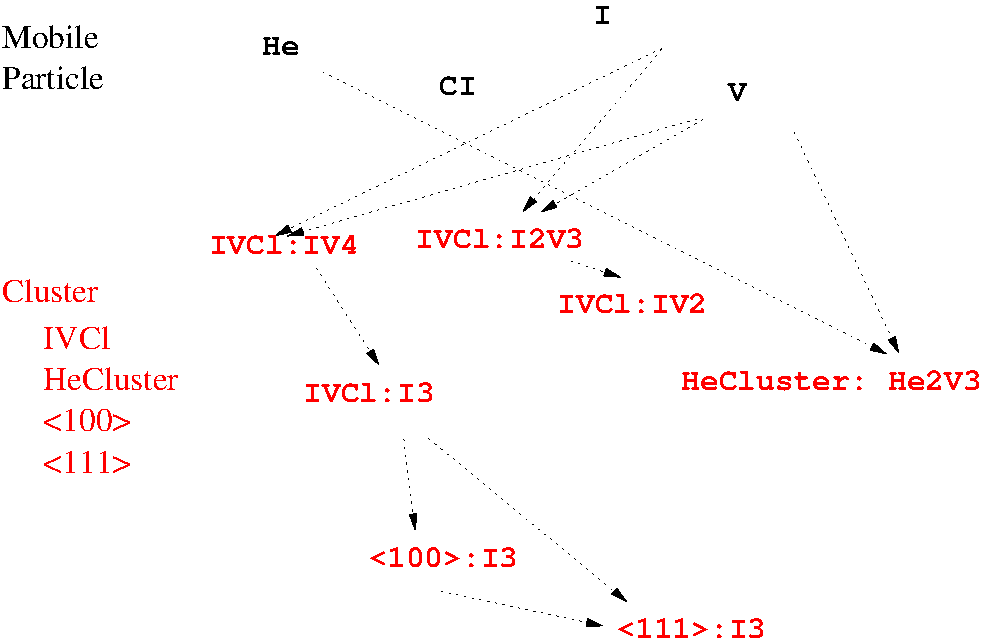
\includegraphics[width=12cm]{images/defect-evolution}
\caption{Different generic defects and their evolution}
\label{fig:defects-evolution}
\end{figure}

Figure~\ref{fig:defects-evolution} shows the generic defect evolution for OKMC simulations in  \MMonCa{}. It starts from point defects, either intrinsic, like interstitials or vacancies, or extrinsic as impurities or dopants. This defects can react between them producing other defective objects. This objects are:
\begin{description}
\item[MobileParticle]\index{MobileParticle} A single particle (point) defect. Migration, \idx{break-up} and FT emission are possible. 
\item[Cluster]\index{Cluster} Anything that is not a mobile particle. It can be extended defects ($I_8$), clusters ($He_4V_5$), combinations ($I_8CP_3$), amorphous pocktes ($I_8V_4$) etc. They can migrate, transform from to other Clusters, trap and re-emit mobile particles, recombine IV pairs and trap other multiclusters. They can have particular shapes. 
\item[Interfaces] \idx{Interfaces} are not formed by particles, although they can contain particles. They are 2D surfaces that separate different materials. They can trap, emit and annihilate particles, and can annihilate clusters. Particle diffusion on the interfaces is also possible.
\end{description}

\section{Definition of defects}
\index{defects!definition}\index{definitions}

The defects being used in the simulation are defined in the \param{Models} file for each material. Description of the important definitions there follow.

\subsection{particles}

Defines the \param{particles} to be used in the material. For instance:
\begin{lstlisting}
map<string,bool> particles { 
	HeI true 
	He  true
	HeV true
	I   true
	V   true
	C   true
	CI  true
	CV  true
}
\end{lstlisting}

\subsection{defined}
\index{defined}
Defines wich generic defects will be used (true/false). There are no reserved words. Any name will be understood as an implemented cluster. For instance, \param{ICluster}, \param{Void}, \param{BICs}, \param{IVCluster}, etc.

An example is
\begin{lstlisting}
map<string,bool> defined { 
	IVCluster true 
	ICluster  true
	VCluster  true
	BICs      true
}
\end{lstlisting}

\subsection{interactions}
\index{interactions}

The parameter \param{interactions} is used to:
\begin{itemize}
\item \index{interaction} Specify whether the interaction between particular defects is allowed or disabled. 
\item \index{capture radius} Specify, optionally, the capture radius for a particular interaction. The interaction will happen when the distance between two particles belonging to each defect is smaller or equal than the specified capture radius. If not specified, the default value of \param{lambda} is used.
\end{itemize}

This parameter requires a list of all possible interactions. Wildcards are allowed for interactions involving \param{Clusters}. The result of interactions allow an optional capture radius for the particular interaction listed. All interactions have the following format:
\begin{lstlisting}
Reactant1+Reactant2  0/true/false/result[,probability][,capture radius]
\end{lstlisting}

The logic for the \idx{reaction syntax} is the following:
\begin{itemize}
\item Reactions between mobile particles giving a particle are defined con true/false.
\item Reactions between clusters, are defined with true/false.
\item Reactions between particles, producing a cluster, are defined with the name of the cluster and the probability to follow that path.
\item In the particular case of reactions between mobile particles producing a recombination, 0 can be specified indicating instant recombination.
\item Reaction between a defect and an interface are specified with true/false.
\item For reactions between particles, particles and clusters, or clusters (i.e., all except interfaces) an optional \idx{capture radius} can be specified.
\end{itemize}

Reactants are the inputs for the \idx{interaction}s.  

The procedure to define interactions, assuming that M is the name of a unary material, is defined in Table~\ref{tab:interactions}.

\begin{sidewaystable}
\caption{Reactions defined in Models/interactions. M represents the material for binary materials, being empty for unary ones. A represents an ``impurity'', an element not constituting the material.}
\label{tab:interactions}
\begin{tabular}{|l|ccl|c||l|}
\hline

Generic &Reactant 1 & Reactant 2 &result& example & comments\\\hline
\hline
MP+MP & MI       & MV       & 0 or MC,prob     & MI+VM IVCluster,1   & 0 means annihilation\\\hline
MP+MP & MI       & MI       & MC,probability   & MI+MI ICluster,0.4  & Total probability should be 1.\\\hline
MP+MP & MV       & MV       & MC, probability  & MV+VM VCluster,1    & Similar to I+I\\\hline
MP+MP & MI or MV & AM       & true             & MI+CM true          & Produces another MP\\\hline
MP+MP & MI       & AV       & true             & MI+HeV true         & Produces another MP\\\hline
MP+MP & MV       & AI       & true             & MV+HeI true,0.3     & A capture radius is specified\\\hline
MP+MP & MI or MV & AI or AV & MC,probability   & MV+CV CCluster,1    & Produces a MC\\\hline
MP+MP & AM       & AI or AV & MC,probability   & CM+CV CCluster,.5   & Produces a MC\\\hline
MP+MP & AV or AI & AV or AI & MC,probability   & HeV+HeV HeCluster,1 & Produces a MC\\\hline
\hline

MC+MP & MC:ID & MP& true/false & HeCluster:He2V2+mI  true     & \specialcell{Wildacards allowed,\\as in HeCluster:*+mI true}. \\\hline
MC+MC & MC    & MC& true/false & HeCluster+HeCluster true,0.5 & \specialcell{All or nothing, with\\a non-standard capture radius}.\\\hline
\hline

MP+Int & MP & Material & true/false & mI+Gas true        & \specialcell{Reactions with an interface\\with the specified material}. \\\hline
MC+Int & MC & Material & true/false & HeCluster+Gas true & \specialcell{Cluster reaction with specified material}.\\\hline
\end{tabular}
\end{sidewaystable}

All the possible interactions, and their capture radius, that can be defined are summed up in Table~\ref{tab:possibleinteractions}. If a \idx{capture radius} is not specified it is taken as the default value of \param{lambda} for the material.

\begin{table}
\caption{Results of the defined interactions}
\label{tab:possibleinteractions}
\begin{center}
\begin{tabular}{|c||c|c|}
\hline
            & \textbf{MP}              & \textbf{MC}  \\\hline\hline
\textbf{MP} & \specialcell{MP MC\\ 0 } & MC           \\\hline
\textbf{MC} & MC                       & MC           \\\hline
\end{tabular}
\end{center}
\end{table}

The interactions are:

\begin{itemize}
\item Mobile particles interact with mobile particles.
\item If a Cluster is formed, the multicluster name and the probability is written (i.e., $<$111$>$,1).
\item If there is a recombination, either 0 or Cluster is written.
\item For MobileParticles, true is written.
\item For interfaces, the interface is written as second reactant: e.g. MI+Gas, $<$111$>$+Gas. They interact with everything.
\end{itemize}



\section{Description of defects and parameters}

\subsection{\tt MobileParticle}
\index{MobileParticle}
MobileParticles are single \idx{point defects}, i.e., they are represented with three coordinates only. They can be either self point defects (interstitials or vacancies) or impurities (carbon, helium, etc). For each impurity or element $A$, a mobile particle with each of the 5 different positions explained in section~\ref{sec:position} can also be found. 

MobileParticle parameters, for a given species $A$ are the following ones:
\begin{description}
\item [A(migration)] An arrhenius with the \idx{diffusivity}.
\item [A(formation)] An arrhenius with the  \idx{formation energy} in the bulk.
\end{description}

The events that a MobileParticle can perform are:
\begin{description}
\item[\idx{Migration}] Standard.
\item[\idx{Break-up}] For instance, $AI \rightarrow AM + MI$, being $M$ the material. The formation parameters are used to define the break-up frequencies, but $E_\mathrm{binding}(AI) = E_f(AM) + E_f(MI) - E_f(AI)$.
\item[\idx{Frank-Turnbull}] For instance, $AM  \rightarrow AI +VM$ or $AM \rightarrow AV + MI$. Formation values are used to compute such break-up frequencies.
\end{description}

If the \idx{charge model} is activated, additional state charges can be defined for each particle. For instance

\begin{description}
\item [AM(state.charge)] AM 0
\item [AI(state.charge)] \verb+AI_0+ 0 \verb+AI_-+ -1
\end{description}

The \idx{levels} in the \idx{band gap} for the transitions between charges have also to be defined.

\begin{lstlisting}
float AI(e(-1,0))   .5
\end{lstlisting}

And, finally, a frequency to \idx{update} the charge state between different states is required.

\begin{lstlisting}
arrhenius AI(update) { 1 0.7 }
\end{lstlisting}


\subsection{\tt Cluster}
\index{Cluster}
Clusters are the agglomeration of any number of impurities with Is or Vs. The first step to include them in a simulation is to allow them in the {\tt Model} file by defining its name. For instance:

\begin{lstlisting}
map<string,bool> defined { 
	IVCluster true 
	ICluster  true
	HeCluster true
}
\end{lstlisting}

Defines 3 {\tt Clusters}: {\tt ICluster}, {\tt IVCluster} and {\tt HeCluster}. 

Once the defects are defined, its implementation is to be written in a file named as the just-defined cluster. Such implementation relies on the following parameters:

All the prefactor units\index{prefactor units} are ``diffusivity'' units (cm$^2$s$^{-1}$). Consequently, they will be transformed into frequency units using the conversion factor $6/\lambda^2$. The lamdba used is not the \param{lambda} defined for each cluster, but the general one in \param{Models/lambda}.

\begin{description}
\item [shape] of the defect, can be {\tt disk}, {\tt plane311}, {\tt irregular} or {\tt sphere}.

\item [to] which defect it evolves. Any valid cluster.

\item [from] which defect it evolved. Any valid cluster.

\item [density.cm2] for {\tt disk} and  {\tt plane311} only. Surface density (atoms/cm$^{2}$).

\item [density.cm3] for {\tt irregular} and {\tt sphere} only. Volumetric density (atoms/cm$^{3}$).

\item [migration.type] for the defect. Could be {\tt 3d}, {\tt parallel} or {\tt perpendicular} to the axis 0 and 1 of the defect.

\item[lambda] used for the defect diffusion. Bigger or smaller lamdbas than the one in \param{Models/lambda} can be used. In particular, use of a bigger lambda will speed up the simulation of cluster diffusion while maintaning the correct diffusivity, but some caution should be taken, because if lambda is too big the cluster might diffuse over particles without reacting with them. Consequently, lambdas bigger than twice the minimum capture distance are not suggested.

\item [axis.0, axis.1] Three axis for the defect. 0 and 1 are the plane for planar defects. 2 is the perpendicular axis to the plane. A {\tt dist}, for instance, will be grown using the axis 0 and 1.

\item [axes.ratio] For {\tt disk} and \{311\} is the geometrical ratio of {\tt axis.0} versus {\tt axis.1}. A value of 2 would mean the defect is twice large in axis 0 than 1.

\item [not.in.plane] Defects are created in the specified plane and all its families. For instance, 1 0 0 will crate also 0 1 0, 0 0 1, defects. If one of these particular planes has to be avoided, it can be specified here. The main use is to avoid defects perpendicular to the surface that will diffuse in 1D parallel to the surface and then will never recombine, slowing down the simulation.

\item[IV.model] True or false. If false, instantaneous recombination of Is with Vs will happen. Otherwise, IV pairs will be maintained and recombined with a specified barrier. Setting this value to true forces to define also an IV.barrier parameter.

\item [formation]\index{formation} The formation energy ($E_f$) of the clusters. The origin of energies is an empty, perfect system. Consequently, formation energy would be the total addition of the formation energies of the isolated, constituent particles, minus the binding energies of each of this particles to the cluster. 

In some cases, the potential energy ($E_p$) might be available. For potential energy if the cluster is something like \verb+An^Im+, the origin of energies ($E=0$) is assumed as a system where all the particles of the cluster exist, but are infinitely separated (i.e., they do not interact). In this case, a system with $n$ AM and $m$ MI. Then, we would have that ($E_f(A_nI_m) = nE_f(AM) + mE_f(MI) + E_p(A_nI_m)$.

The procedure should returns a list with all the cluster IDs and its formation energies. This list is used as the existing clusters later. For instance, if CCluster is defined as a cluster and we want to have 3 clusters (\verb+C2^I+, \verb+C^I2+ and \verb+C2+), formation should return something like {\tt \verb+C2^I -2 C^I2 -1 C2 .3+}.

This parameter is of extreme importance because it also defines the available clusters. If a cluster is not defined here, but in other parameters, \MMonCa\ will ignore it. If a cluster is defined here but not in other parameters, \MMonCa\ will assume default values for the non-defined cluster in the other parameters. Formation, then, is the ``canonical'' definition of available clusters, for both types and syntaxis.

\item [prefactor]\index{prefactor} The emission prefactor for each emitted particle. The cluster is written first, and the emitted particle is attached with a comma. For instance, emission of MI from \verb+C^I2+ would be {\tt \verb+C^I2,MI+}. Creation of FPs is allowed, and also controlled with the prefactor (and the opposite reaction). For instance, He5 $\rightarrow$ He5V + MI. Since this is an I emission, the prefactor would be {\tt He5V,MI}. A list with all the clusters and all the possible emissions is expected. If some prefactor for a cluster defined in the formation is missing, the code assumes its prefactor is 0.

\item [percolation]\index{percolation} Boolean parameter to allow the reaction of a cluster with another one while growing, and without the need of diffusion (i.e., without needing one cluster moving into the other).

\item [transform.to] Procedure that returns the rates for transforming the defect to {\tt to }. A list with all the clusters with the prefactors and energies is expected. If a cluster is not included, its Tranformation rate is ``0 5'', i.e., no transformation.

\item [transform.from] Procedure that returns the rates for transforming the defect to {\tt from}.  A list with all the clusters with the prefactors and energies is expected. If a cluster is not included, its transformation rate is ``0 5'', i.e., no transformation.

\item [migration]\index{migration} Migration energy of the cluster, as an arrhenius value (prefactor and activation energy).  A list with all the clusters with the prefactors and energies is expected. If a cluster is not included, its transformation rate is ``0 5'', i.e., no migration.

\item[IV.barrier] Procedure that returns the rates for recombination of IV pairs. If a cluster is not included, the rate is ``0 5'', i.e., no recombination.

\end{description}

All these parameters are defined with a key and a value. The keys used in {\tt formation} are used in the other procedures. Different notations might be available for the same cluster, as explained in sec.~\ref{sec:syntaxis}, but we strongly suggest being consistent with the one chosen. The parameters with procedures are described in Table~\ref{tab:multicluster}

\begin{table}
\caption{Keys and values needed to defined clusters}
\label{tab:multicluster}
\begin{tabular} {l|ll|rr|c}
\hline
Parameter name & key              & value     & key example   & value example & default\\\hline
formation      & cluster          & float     & CV2           & -2.4          & NO \\
prefactor      & cluster,particle & float     & CV2,V         & 1e-3          & 0 \\
migration      & cluster          & arrhenius & CV2           & 0.01 1.2      & 0 5\\
transform.to   & cluster          & arrhenius & CV2           & 1e-3 .7       & 0 5\\
transform.from & cluster          & arrhenius & CV2           & 1e-3 .5       & 0 5\\
IV.barrier     & cluster          & arrhenius & \verb+CV2^I+ & 1e-2 .4       & 0 5\\
\end{tabular}
\end{table}

For instance, for a hypothetical carbon cluster defined in silicon:

\begin{lstlisting}        
string shape           	irregular
float density.cm3      	5e22
string to    			CCluster
string from  			CCluster
string migration.type	3d
// coordinates axis.2   1 0 0
coordinates axis.1     	0 1 0 
coordinates axis.0     	0 0 1
coordinates not.in.plane 0 0 0
float       axes.ratio 	1
float       lambda 0.387

bool IV.model false
proc transform.to   { return "" }
proc transform.from { return "" }
proc migration      { return "" }

proc formation {
    set EfC 0
    set EfI 3.6
    set list ""
    
    append list "C2I   [expr 2*$EfC + 1*$EfI -2.3] "
    append list "C2    [expr 2*$EfC + 0*$EfI -1.2] "
    append list "C2I2  [expr 2*$EfC + 2*$EfI -7] "
    append list "C3I   [expr 3*$EfC + 1*$EfI -1.7] "
    append list "C3I2  [expr 3*$EfC + 2*$EfI -9.7] "
    append list "C3I3  [expr 3*$EfC + 3*$EfI -11.5] "
    append list "C4I3  [expr 4*$EfC + 3*$EfI -13.7] "
    append list "C4I4  [expr 4*$EfC + 4*$EfI -16.5] "
    append list "C4I2  [expr 4*$EfC + 3*$EfI -12.5] "
    append list "C5I3  [expr 5*$EfC + 4*$EfI -13] "
    append list "C5I4  [expr 5*$EfC + 4*$EfI -20.5] "
    append list "C5I5  [expr 5*$EfC + 5*$EfI -25.0] "
    append list "C6I5  [expr 6*$EfC + 5*$EfI -26.9] "
    append list "C6I4  [expr 6*$EfC + 4*$EfI -25.4] "
    append list "C6I6  [expr 6*$EfC + 6*$EfI -30.9] "
    return $list
}

proc prefactor {
     set list ""
     append list "C2I,SiI   2.03e-2 "
     append list "C2I,CI    2.03e-2 "
     append list "C2I,VSi   2.03e-2 "
     append list "C2,SiI    2.03e-2 "
     append list "C2,CI     2.03e-2 "
     append list "C2I2,VSi  2.03e-2 "
     append list "C2I2,CI   2.03e-2 "
     append list "C3I,SiI   2.03e-2 "
     append list "C3I,CI    2.03e-2 "
     append list "C3I2,SiI  2.03e-2 "
     append list "C3I2,CI   2.03e-2 "
     append list "C3I2,VSi  2.03e-2 "
     append list "C3I3,VSi  2.03e-2 "
     append list "C3I3,CI   2.03e-2 "
     append list "C4I3,SiI  2.03e-2 "
     append list "C4I3,SiI  2.03e-2 "
     append list "C4I3,CI   2.03e-2 "
     append list "C4I2,CI   2.03e-2 "
     append list "C4I2,SiI  2.03e-2 "
     append list "C4I4,CI   2.03e-2 "
     append list "C4I4,VSi  2.03e-2 "
     append list "C5I3,SiI  2.03e-2 "
     append list "C5I3,CI   2.03e-2 "
     append list "C5I4,SiI  2.03e-2 "
     append list "C5I4,VSi  2.03e-2 "
     append list "C5I4,CI   2.03e-2 "
     append list "C5I5,CI   2.03e-2 "
     append list "C5I5,VSi  2.03e-2 "
     append list "C6I5,SiI  2.03e-2 "
     append list "C6I5,VSi  2.03e-2 "
     append list "C6I4,CI   2.03e-2 "
	
     return $list
}
\end{lstlisting}

Finally, for a cluster with a {\tt IV.model} set to true, an extra producedure would be required.

\begin{lstlisting}
proc IV.barrier {
 set prefactor   5.0e-4
 set energy(1)   0.43
 set energy(2)   0.7
 set energy(199) 1.6
 set energy(255) 2.7
 set alpha       1.0
 
 set list ""
 for { set size 0 } { $size < 50 } { incr size } {
     for { set iv 1 } { $iv < 250 } { incr iv } {
	 set pref [expr ($prefactor*pow($iv,$alpha))]
	 set ener $energy(255)
	 
	 if { $iv <= 1 } { set ener $energy(1) }
	 if { $iv == 2 } { set ener $energy(2) }
	 if { $iv <= 199 && $iv > 2 } {
	     set b [expr ($energy(199) - $energy(2))/(199. -2.)]
	     set a [expr $energy(199) - $b*199.]
	     set ener [expr $a + $b*$iv]
	 }
	 if { $iv <= 255 && $iv > 199 } {
	     set b [expr ($energy(255) - $energy(199))/(255. -199.)]
	     set a [expr $energy(255) - $b*255.]
	     set ener [expr $a + $b*$iv]
	 }	
	 lappend list V$iv^I[expr $size+$iv]
	 lappend list $pref
	 lappend list $ener
	 lappend list V[expr $size + $iv]^I$iv
	 lappend list $pref
	 lappend list $ener
     }
   }
   return $list
\end{lstlisting}

\subsubsection{Cluster interactions}

The result of the interactions between clusters needs to be defined in an array of strings names {\tt interaction.result} placed in the {\tt Models} file for each material. Every line in the array must contain 5 arguments in the form \verb+ reactant1 operator reactant2 = result+.
\begin{description}
\item [reactant1] Type of the first interacting defect. (For instance, ICluster)
\item [reactant2] Type of the second interacting defect. (For instance, $<$111$>$)
\item [operator] An operator to take the defect sizes ($s_1$ and $s_2$, counted as the total number of particles) into account. One of the following:
  \begin{description}
    \item [+] To specify the result independently on the size of both reactants.
    \item [==] When one reactant has the same size as the other. ($s_1 = s_2$)
    \item [$\sim$=,n] When one reactant is approximately the same size as the other, measured as $$|s_1 - s_2|/\mathrm{max}(s_1,s_2) < n$$.
    \item [$<$] When $s_1 < s_2$.
    \item [$>$] When $s_1 > s_2$.
  \end{description}
Only one reaction for each case has to be specified. For instance \verb+<111> > <100> = <111>+ also implies that \verb+<100> < <111> = <111>+, but this last one does not need to be specified. If a reaction is specified several times, a warning will be issued and the last reaction will be taken only.
\item [result] Name of the resulting defect. (For instance, $<$111$>$)
\end{description}

\marginpar{Example}

\begin{lstlisting}
array<string> interaction.result {

        ICluster + ICluster = ICluster
        ICluster + <100> = <100>
        ICluster + <111> = <111>      
        VCluster + VCluster = VCluster
        <100> + <100> = <100> 

        <100> ~=,.05  <111> = <100>
        <100> >   <111> = <100>
        <100> <   <111> = <111>

        <111> ~=,.05 <111> = <100>
        <111> >  <111> = <111>        
        <111> <  <111> = <111>        

        VCluster == <100> = <100>
        VCluster < <100> = <100>
        VCluster > <100> = VCluster

        VCluster == <100> = <100>
        VCluster == <111> = <111>
        VCluster < <111> = <111>
        VCluster > <111> = VCluster

        VCluster == ICluster = VCluster
        VCluster >  ICluster = VCluster
        VCluster <  ICluster = ICluster
}
\end{lstlisting}

\subsubsection{Summary}

Clusters in \MMonCa\ are very flexible defects. They can be used as multi clusters for activation deactivation of defects (i.e., BICs and similar in semiconductors), to simulate bubbles (HeClusters in metals) extended defects (\{311\}, $<$111$>$, etc...) and amorphous pockets (\verb+V2I+ etc...).

Clusters can migrate, transform, emit constituent particles and recombine existing IV pairs. Clusters can adopt different shapes, and interact between them.


\subsection{Interfaces}
\index{Interfaces}

An interfaces is a defect between materials with different properties, or between a material and the lack of it (a free interface).

\subsubsection{Parameters}

Interface defects are not user-specified. They are build by default between materials with different names. For a free interface, the special material \param{Gas} can be used. 

Because an interface involves two materials, the interface parameters are defined in folders that are created by appending the name of both materials separated with an underline ``\verb+_+'', in alphabetical order. This way, an interface between Iron and Gas would be parametrized under the {\tt Gas\verb+_+Iron} name.

Each material folder contains the parameters for each element that can interact with the interface. The parameters allowed for these elements are listed below. The parameter \param{left} is important, because it defines what is called ``left'' in the parameters using it. This way, if \param{left} is set to ``Iron'', any param finishing in ``left'' will refer to ``Iron'', and ``right'' will refer about the other material in the interface, independently on the name of the folder. 

For instance, in {\tt Iron\verb+_+Gas} if \param{left} is Iron, then any reference to ``right'' will refer to Gas. In {\tt Copper\verb+_+Iron}, if \param{left} is also Iron, ``right'' will mean Copper. As you can see, this is independent on whether the folder name (ordering the names alphabetically) starts or finishes with Iron.

\begin{description}
\item[\param{barrier.left}] The (extra) energetic barrier to be overcome to react with the interface.
\item[\param{barrier.right}] See barrier.left.
\item[\param{desorption.high}] See desorption.threshold.
\item[\param{desorption.low}] See desorption.threshold
\item[\param{desorption.threshold}] For surface concentrations lower than this value, the parameter \param{desorption.low} will be used. Otherwise \param{desorption.high} will be applied. Desorption is the probability for a particle to be annihilated at the surface.
\item[\param{formation}] The formation energy of the impurity when trapped at the interface. The particle will be emitted to either side depending on the difference of energies between this formation energy and the formation energy in the materials at either side.
\item[\param{left}] Definition of which material is considered left, independently on the name of the folder for the interface.
\item[\param{migration}] Migration energy and prefactor for the inpurity on the interface.
\item[\param{recombination.lenght.left}] For self-interstitials and self-vacancies, defines the sink efficiency at the interface.
\item[\param{recombination.lenght.right}] See recombination.lenght.left.
\end{description}

A graphical description of the meaning of these parameters can be seen in Fig.~\ref{fig:interface}

\begin{figure}
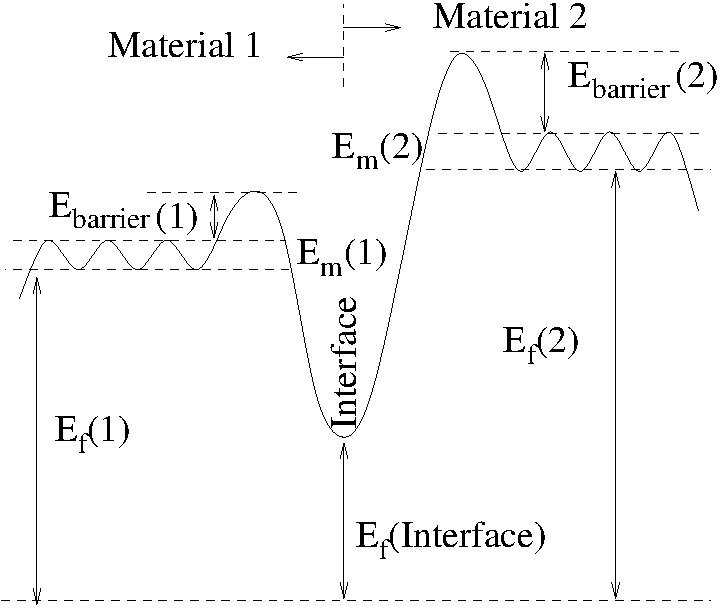
\includegraphics{images/interface}
\caption{Energies involved at the interface reactions.}
\label{fig:interface}
\end{figure}


\subsubsection{Interactions}

The interactions with interfaces are defined in the {\param Models} file for each side of such interface. The syntax for them is
\begin{lstlisting}
Defect+MaterialFullName true/false
\end{lstlisting}
the full name for the material is to be used. This way the syntax checker can distinguish between the interaction with an interface (for instance, {\tt I+Iron}, or with an impurity of the same material {\tt I+Fe}.


As an example, in the case of a {\tt Copper\verb+_+Iron} interface, at the {\tt Iron} side, the interaction with the material  is defined at {\tt Iron/Models/interactions} as
\begin{lstlisting}
Defect+Copper true
\end{lstlisting}
being {\tt Defect} the defect being considered (I, V, ICluster, etc...). Similarly, at the Copper side we will see
\begin{lstlisting}
MP+Iron true
\end{lstlisting}

\subsubsection{Conclusions}
Interfaces are 2D planar objects isolating one material from a different one. Mobile particles and clusters are allowed to interact with them. For mobile particles, they can be annihilated, or trapped and re-emitted to either side. For clusters they can only be annihilated (desorption). 



\section{Amorphization}
\index{amorphization}
\label{sec:amorph}

When a region of the material overcomes a certain threshold of damage concentration (i.e. self-interstitials and vacancies), that region is amorphized, so all the atoms from the material are displaced from their crystalline position, and no more damage can be introduced in those areas. Self-interstitial and vacancy definitions no longer make sense in those areas. Such threshold value is defined in the {\tt Models} file for each material. 

\begin{description}
\item [amorphization.threshold=$<$value$>$] Units are atoms/cm$^3$ units. To deactivate the amorphization model, it is enough to not assign a value to it.
\end{description}

If the amorphization model is wanted to be active, the definition of the amorphous material corresponding to the crystalline one needs to be defined. For example, to active the amorphous model in the material {\tt Silicon} , {\tt AmorphousSilicon} must be defined.

When amorphizing an area of the simulation, the {\tt LKMC} module is called, and lattice atoms are placed on the interfaces between amorphous and crystalline zones. This is done dynamically when using {\tt cascade} or {\tt profile} commands. When new areas are amorphized, lattice atoms are automatically removed in areas where the amorphous/crystalline interfaces no longer exist. 

For output information of this model, see section \ref{sec:extract}.




\chapter{Lattice KMC: Lattice atoms}
\index{LKMC}

\section{Introduction}

\MMonCa\ contains a module to perform Lattice KMC simulations. Such module can be used independently or linked to the Object KMC module. 

The basis of a Lattice KMC simulation is the ``Lattice Atom''. A lattice atom is a representation of a real atom in the lattice of a crystal, or a position of such atom if it had to be in the lattice. Depending on the local configuration and other material properties (temperature, concentrations, deformations), different events are associated with the lattice atom. The main event to be associated is the ``filling'' of such position, if its represents an empty position. 

Using such a simple approach, two different \index{epitaxy} epitaxies can be simulated:
\begin{description}

\item[Solid Phase Epitaxial Regrowth] or SPER, where a crystalline phase advances against an amorphous phase. In this case the ``filling'' is interpreted as an atom in the amorphous phase attaching to a crystalline position, and thus being incorporated to the crystalline phase. More information on these type of models can be found in Refs.~\cite{MARTIN-BRAGADO-APL09,MARTIN-BRAGADO-APL11,MARTIN-BRAGADO-JAP12}.

\item[Solid Gas Epitaxy] The epitaxial growth of a material by reactions with existing gases, for instance, Selective Epitaxial Growth. For this models, the ``filling'' of a Lattice Site is directly related to the deposition of a new atom on the interface. An example can be found in Ref.~\cite{MARTIN-BRAGADO-APL11b}. These type o models can also include different mechanisms: diffusion, etching, deposition, etc. An example of such a model is found in Ref.~\cite{CHEN-SISPAD13}.
\end{description}



\chapter{Output}

\section{Updates}
\index{updates}

\MMonCa\ uses an update mechanism to call update events (to be described later) based on the following parameters:
\begin{description}
\item[time.decade\index{time.decade}] The update event wil be called this number of times per decade of simulated time. For instance, a value of 10 here will update at times 1, 2, 3, 4, 5, 6, 7, 8, 9, 10, 20, 30, 40, 50, 60, 70, 80, 90, 100, 200, ...
\item[time.delta\index{time.delta}] The update event will be called at the specified interval. For instance, for {\tt time.delta}=5, at 5, 10, 15, 20, ...
\item[time.min\index{time.min}] Minimum time to start the updates.
\item[events\index{events}] The update event will be called each {\tt events}.
\end{description}

All the above options work at the same time. For instance, it is possible to have the updates 3 times per decade, and also every 10 seconds.

These update mechanisms are used for the following modules:

\begin{description}
\item[snapshots\index{snapshot}] \MMonCa\ outputs the status the simulation with a frequency specified in the {\tt MC/General/snapshot} update. This update produces two different actions. First, it outputs the current status, and it also calls the {\tt snapshot} procedure. The user can defined a snapshot procedure to extract information, save the time evolution of the simulation, etc. The option {\tt events} does not work for snapshots.
\item[charge model update\index{update!charge model}] The frequency at which the Poisson solver is called is specified in the {\tt MC/Electrostatic/update} parameter.
\item[mechanical update\index{update!mechanical}] The frequency at which the mechanical solver is called and the mechanical information fed into KMC is specified in the {\tt Mechanics/General/update} parameter.
\end{description}




\section{Obtaining output}
\index{output}

The two commands mostly used to obtain information from a \MMonCa\ simulation are:
\begin{description}
\item[extract\index{extract}]  It extracts profiles, concentrations, defect numbers, etc... in plain ASCII text. See~\ref{sec:extract}.
\item[save\index{save}] It saves the atomistic information in {\tt xyz} or {\tt ovito} format for visualization. See~\ref{sec:save}.
\end{description}

Extract can collapse the information in 1, 2 and 3 dimensions with the use of the {\tt dimension}\index{dimension} option.


\chapter{Commands}
\label{chap:commands}

All the commands can use the generic option \param{no.print} when you do not want \MMonCa\ to print out the command line.

\section{anneal}
\index{anneal}

Anneals the simulation at the requested temperature in Celsius degrees. Different criteria to exit the anneal are {\tt depth}, {\tt events} or {\tt time}.

\begin{description}
\item [depth=$<$depth$>$] Specifies recrystallized depth, in nm, as the exit criteria.
\item [epitaxy="list"] Specifies, in ``list'', a map of gas names and partial pressures, used for epitaxy.
\item [events=$<$events$>$] Specifies a number of simulated events as the exit criteria.
\item [log=$<$filename$>$] Specifies the name of a file to log a list of simulated events and time every 100 events. (This list can be quite big).
\item [temp=$<$temperature$>$] Requested temperature in Celsius degrees.
\item [time=$<$time$>$] Specifies simulated time, in seconds, as the exit criteria.
\end{description}

This command prints an information line at a rate of 10 snapshots per decade, i.e., at 1,2,3... 10,20,30... 100,200... After priting the line, the procedure  \param{snaphot} is called to perform user-defined actions. Such procedure can be used, for instance, to save the simulation.

\begin{lstlisting}
proc snapshot { } {
	save ovito=evolution append
}
\end{lstlisting}

\subsection{Examples}
\begin{itemize}
\item \verb+anneal temp=600 time=20+
\item \verb+anneal temp=600 depth=20+
\item \verb+anneal temp=300 time=0.5 events=1000000+
\item \verb+anneal temp=700  time=1 epitaxy="Si 1 Ge 0.5"+
\end{itemize}

\section{cascade}
\index{cascade}

Command used to implant or insert cascades of point defects into the simulation. Mostly used for damage simulation from an external source.

The global options for all {\tt cascade} commands are

\begin{description}
\item[correct.for.surface]\index{correct.for.surface} Option to change the depth coordinate and adapt it to the place where the surface is. It assumes the cascades are computed for a surface at $x=0$.
\item[defects]\index{defects} Procedure used to obtain the defect type of clusters. i.e., Is V4 a ICluster, a 111, etc.
\item[fluence]\index{fluence} Fluence for cascades in the simulation. The number of cascades will be $A\mathrm{fluence}$ being $A$ the $YZ$ simulation area. Compulsory. Units: cm$^{-2}$.
\item[do.not.react]\index{do.not.react} If specified, the new incoming particles will not react with the existing ones.
\item[do.not.shift]\index{do.not.shift} For file cascades only: do not change the y and z coordinates of the read cascade: use it as it is.
\item[flux]\index{flux} Optional option to specify the rate at which cascades will be annealed. If not specified, cascades will be assumed to be ``instantaneous''
\item[periodic]\index{periodic} If present, this flag allows for coordinates outside the simulation cell to be reinserted by means of periodic boundary conditions.
\item[temp]\index{temp} Optional. Temperature in Celsius degrees to anneal the cascades (to simulate dynamic annealing). If not specified, it is the current simulation temperature.
\item[voluminic]\index{voluminic} Optional. If present, this flag allows to introduce the cascades homogeneously in the volume of the sample instead of just in the surface.
\end{description}

The command \param{cascade} will introduce the cascades one by one in the simulator and perform a ``dynamic annealing'' of $-\Delta t\log(r)$ after each cascade. $r$ is a random number between 0 and 1, and $\Delta t$ is the average time between cascades, equals to \param{fluence}/\param{flux}.

The currently supported models for cascades are:
\begin{description}
\item [file] The only supported source of cascades now: Read them from a file.
\end{description}

The following options are valid for \param{file} only.

\begin{description}
\item[file=$<$filename$>$] Name of the input file. Compulsory.
\item[format=$<$formattext$>$] Optional format of the input file. It uses A:B:C:D if not specified.
\end{description}

Cascade accepts two different formats, called ``New cascade'' and ``Number of particles''. The general format of the input file is the same, the only difference is the label used to indicate when a new cascade starts. \MMonCa\ detects the format automagically.
\begin{itemize}
\item A file can contain several cascades. Thus, it is necessary to insert some special label in the cascade file every time a new cascade starts.
\item Each cascade starts with one of this two formats:
\begin{description}
\item[\# New cascade] The verbatim label \verb+# New cascade+. 
\item[Number] A number indicating how many defects (one per line) are contained in each cascade.
\end{description}
\item After the special label, the list of point defects follows.
\item The format for each line in the list of defects must be the same, and it has to contain, at least, the name of the point defect, and three columns with  the x, y and z coordinates. The $y$ and $z$ of such coordinates refer to an impact point of $(0,0)$.
\end{itemize}

The \param{cascade} command will read as many cascades as needed, in the order they have in the file, and shift them with random $y$ and $z$ numbers to fill the whole area. If more cascades than the ones specified in the file are needed the process will start again from the first cascade in the file.

The \param{format} command needed for the \param{file} option specifies the format for the point defects in the file. It is a string containing a list of field. Such list of fields is separated by colons ``:''. 4 fields are needed, representing the particle type (mobile particle types only) and the x, y and z coordinates in nanometers. The positions of such fields in this order will be indicated by using the letters A to Z. Arithmetic operations are possible. The letters A to Z represent the column number in the text file specified in the \param{filename}. Some examples follow.

The \param{defects} option allows the specification of a procedure to resolve the defect type of a given cluster:
\begin{lstlisting}
proc defects { def } { 
	if { [string index $def 0] == "V" } 
		return "VCluster" 
	return "<111>" 
}
\end{lstlisting}

\subsection{Cascade examples}
\index{cascade!formats}
Two equivalent examples are given above in the two accepted formats. The format is automatically detected by \MMonCa.

\subsubsection{Format ``\# New cascade''}

The following example contains 2 cascades:

\begin{lstlisting}
# New cascade
I 23.4 .5  .9
V 21.2 .6  .85
I 17.2 .55 .92
V 18.0 .53 .87
I 20.0 .58 .91
# New cascade
I 19.9 -.1 .1
V 19.7 -.2 .2
I 17.2 .1  -.1
V 19.3  .2 .2
I 18.3 -.14   .17
V 20.1 -0.03 0.1
I 21.9  0.12 0.16
\end{lstlisting}

\subsubsection{Format ``number of defects''}

The following example contains 2 cascades:

\begin{lstlisting}
5
I 23.4 .5  .9
V 21.2 .6  .85
I 17.2 .55 .92
V 18.0 .53 .87
I 20.0 .58 .91
7
I 19.9 -.1 .1
V 19.7 -.2 .2
I 17.2 .1  -.1
V 19.3  .2 .2
I 18.3 -.14   .17
V 20.1 -0.03 0.1
I 21.9  0.12 0.16
\end{lstlisting}

\subsection {Examples}

Some examples for the \param{format} field follows:
\begin{itemize}
\item \verb+A:B:C:D+ A file in nanometers where the first column are the particles types and the following ones x, y and z.
\item \verb+A:C:D:E+ A file, in nanometers, where the first column are the particle types and the x, y and z are codified in 3$^\mathrm{rd}$, 4$^\mathrm{th}$ and 5$^\mathrm{th}$ columns. The second column in the file is not used.
\item \verb+D:A*1e7:B*1e7:C*1e7+ A file, where x,y and z are in the first, second and third column and are specified in cm (being converted into nm by using the factor $10^7$. The fourth column contains the particle types.
\item \verb-A:B+C*10:B+C*10:B+C*10- In this file, the x, y and z coordinates are going to be the same: the second column plus then times the third one.
\end{itemize}

Some examples for the whole command follows:
\begin{itemize}
\item \verb+cascade file=cascade periodic fluence=5e14 flux=1e12 temp=-150+
\item \verb+cascade file=cascade periodic fluence=5e14 temp=-150 voluminic+
\item \verb-cascade file=cascade format=B:C*.287:D*.287:E*.287 periodic fluence=4.8e9-
\end{itemize}

\section{extract}
\index{extract}
\label{sec:extract}

It extracts simulation information. It does not write information on screen, but returns it as a variable. If you want to see something on screen, use the \param{lowmsg} command to print it.

\begin{description}

\item [ac.coverage]\index{ac.coverage} Returns the surface hydrogen coverage in epitaxial models, as a $[0-1]$ value (ML or monolayer).

\item [ac.max]\index{ac.max} Returns a list with the maximum values for the Lattice KMC interface position in x, y and z. Accepts the optional arguments  \param{min.x=$<$minx$>$}, \param{max.x=$<$max.x$>$}, \param{min.y=$<$miny$>$}, \param{max.y=$<$max.y$>$},  \param{min.z=$<$minz$>$} and \param{max.z=$<$max.z$>$} to limit the extraction domain size. 

\item [ac.mean]\index{ac.mean} Returns a list of the mean value of the Lattice KMC interface position in x, y and z respectively. Accepts the optional arguments  \param{min.x=$<$minx$>$}, \param{max.x=$<$max.x$>$}, \param{min.y=$<$miny$>$}, \param{max.y=$<$max.y$>$},  \param{min.z=$<$minz$>$} and \param{max.z=$<$max.z$>$} to limit the extraction domain size. 

\item [ac.min]\index{ac.min} Returns a list with the minimum values for the Lattice KMC interface position in x, y and z. Accepts the optional arguments  \param{min.x=$<$minx$>$}, \param{max.x=$<$max.x$>$}, \param{min.y=$<$miny$>$}, \param{max.y=$<$max.y$>$},  \param{min.z=$<$minz$>$} and \param{max.z=$<$max.z$>$} to limit the extraction domain size. 

\item [ac.stdev]\index{ac.stdev} Returns a list of the standard deviation of the Lattice KMC interface in x, y and z respectively. Accepts the optional arguments  \param{min.x=$<$minx$>$}, \param{max.x=$<$max.x$>$}, \param{min.y=$<$miny$>$}, \param{max.y=$<$max.y$>$},  \param{min.z=$<$minz$>$} and \param{max.z=$<$max.z$>$} to limit the extraction domain size. 

\item [amorphous.fraction]\index{amorphous.fraction} Returns the fraction of space that is amorphous in an {\tt OKMC} enviroment for the material specified in the required option \param{material=$<$mt$>$}. For more information, read Section \ref{sec:amorph}.

\item [coord=$<$x y z$>$]\index{coord} Uses the coordinate x, y and z as the starting center to look for neighbors in the \param{coordination} command.

\item [coordination]\index{coordination} Returns a list of neighbors, distance to it, the neighbor type and total account of neighbor types. It requires the use of the option \param{coord} to specify the value of the coordinate to use as a center and \param{radius} for the look-up radius. It buils a crystal as a sphere with the specified radius plus 0.5 nanometers, so the specified coordinate should be close to 0 0 0.

\item [count.defects]\index{count.defects} Returns how many defects are in the simulation. It accepts the following options to ``filter'' the results: \param{material} for a particular material, \param{name} to specify a particle name, \param{defect} for a defect name, \param{min.size} for a minimum size and \param{ID} for a particular defect type.

\item [count.particles]\index{count.particles} Returns how many particles are in the simulation. It accepts the following options to ``filter'' the results: \param{material} for a particular material, \param{particle} to specify a particle name, \param{defect} for a defect name, \param{min.size} for sizes equal or bigger and \param{ID} for a particular defect type. It is different from \param{count.defects}. For instance, a B2I3 cluster will return 3 interstitial particles, but only 1 defect.

\item [count.positions]\index{count.positions} Returns how many particles are in a particular position. It requires the argument \param{position}\index{position} and accepts the argument \param{material} to filter the particles to the specified material. 

\item [defect]\index{defect} Parameter used by \param{histogram} to specify the defect type. Also used by \param{profile} to restrict the output to a particular cluster.

\item [defect.radius]\index{defect.radius} It computes the average radius (in nm) of the specified defects. It requires the parameter \param{defect} and accepts the optional parameters \param{ID} to specify a particular type and \param{min.radius} to set up a threshold that defines when a defect is ``visible'' and will be included in the calculation.

\item [defects=$<$list$>$]\index{defects} Returns all the defects (OKMC particles) and positions in the simulation. If all the defects are requested, an empty list (defects=\{ \}) is to be provided. Otherwise, an enumeration of the defects requested, separated by spaces, is to be provided. For MobileParticles, \param{MobileParticle} has to be specified. For other defects, the defect name (eg. \param{ICluster}, \param{VCluster}) is to be written. If alloy atoms are requested, type \param{Alloy}.

\item [diffusivity]\index{diffusivity} Returns the diffusivity of the specified particle \param{name} in the specified  \param{material}. It does not work for I or V particles. If \param{macroscopic} is specified, then it tracks the diffusivity of the whole family of particles associated. Use \param{extract reset} to start measuring.

\item [dimension]\index{dimension} Sets the dimension to collapse the output. Accepts 0, 1 2 and 3. If 0 is specified, no geometrical information is obtained, just a value with the overall mean value.

\item [dose]\index{dose} Extracts the damage recieved by the material by the \param{cascade} command. The units are in dpa. This command assumes that the cascades contain Frenkel pairs, that is, same number of interstitials and vacancies (accepts clusters but the total ammount of interstitials and vacancies must remain equal), if not this command will give an underestimated or overestimated dpa value.

\item [histogram]\index{histogram} Requires the parameters \param{defect} and \param{material}. Returns a histogram for the given defect/s name. Several defects can be used separated by commas, for instance {\tt ICluster,VCluster}. A histogram is considered a list of cluster names and the number of them present when issuing the command. 

\item [file=$<$filename$>$]\index{file} This option can be added to {\em any} of the previous parameters to write the results in filename.

\item [fuzz]\index{fuzz} Returns a ``y z depth'' array listing all the depths at which a free interface was detected.

\item [jumps]\index{jumps} Returns the number of jumps for the mobile particle specified in the required option \param{name=$<$pt$>$}

\item [min.radius]\index{min.radius} Optional parameter for \param{defect.radius}. It considers only ``visible'' defects with radius equal or bigger than the specified one.

\item [min.size]\index{min.size} Optional parameter for \param{count.defects} or \param{count.particles}. It limits the count to defects with size equals or bigger than the specified. The size of a defect is defined as its total number of particles.

\item [profile]\index{profile} Returns the concentration for the particle specified in the required option \param{name=$<$pt$>$}. When simulating binary alloys it is possible to extract the atom counters of the A and B species in the AB binary alloy with the \param{name=A.atoms} and \param{name=B.atoms} respectively. Also it is possible to extract the profile of the A atoms of the AB binary alloy by no introducing the \param{name} keyword and introducing the desired material profile with the \param{material} keyword. LKMC information can also be extracted through \param{name=lkmc.defects} and \param{name=lkmc.ac} options and corresponding to defective configurations and amorphous/crystalline interface respectively.

\item [profile.damage]\index{profile.damage} Returns the damage concentration (i.e. self-Interstitials and Vacancies) for the material specified in the required option \param{material=$<$mt$>$}. Such concentration saturates at the {\tt amorphization.threshold} value. For more information, read Section \ref{sec:amorph}.

\item [profile.mobile]\index{profile.mobile}  Returns the mobile concentration for the mobile particle specified in the required option \param{name=$<$pt$>$}. It assumes $[X] = \mathrm{jumps} / (\Delta t \Delta V \nu(pt))$.

\item [reset]\index{reset} Resets the information for mobile particles. It allows incremental displays of properties for mobile particles. If \param{reset} is not used, then all the properties for mobile particles are accounted from the very beggining of the simulation, otherwise, the magnitudes are an average between the last reset and the current time.

\item [strain.xy] Returns the shear strain (xy) loaded into OKMC in a 2D X/Y projection.

\item [time]\index{time} Returns the current simulated time.

\end{description}

\subsection{Examples}
\begin{itemize}
\item \verb+extract count.particles defect=ICluster+ Extracts how many particles are in "ICluster"
\item \verb+extract count.particles defect=VCluster ID=V3+ Extracts how many particles are contained in V3 in "VCluster".
\item \verb+extract diffusivity macroscopic name=He material=Copper+
\item \verb+extract time+
\item \verb+extract ac.mean+ Extracts a list containing the x, y and z mean values of amorphous/crystalline interface positions. Use \verb+[lindex [extract ac.mean] 0]+ to extract the x mean value.
\item \verb+extract histogram defect=<111> material=Iron+ 
\item \verb+extract profile name=Cr dimension=1 material=Iron+ Extracts the profile [$cm^{-3}$] of the Cr atoms collapsed to the X-dimension
\item \verb+extract profile material=Iron+ Extracts the profile [$cm^{-3}$] of the Iron lattice atoms (computed from the cell counters)
\end{itemize}

\section{init} \label{sec-Commands-init}
\index{init}

Defines the simulation cell sizes and the material specification to be used.

\begin{figure}
\begin{center}
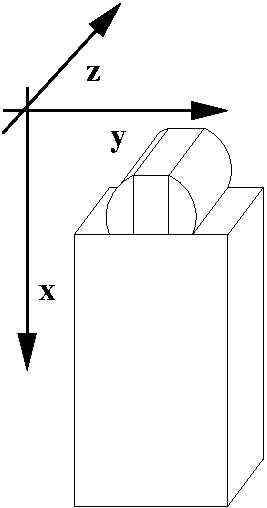
\includegraphics{images/axes}
\caption{Definition of axes in MMonCa}
\end{center}
\label{fig:axes}
\end{figure}

\subsection{Uniform mesh specified using minimum and maximum}

\begin{description}
\item [material=$<$procedure$>$] Specifies the name of a procedure where \MMonCa{} will obtain the material information. The procedure has three input arguments, x, y and z, and returns the name of a valid material.
\item [maxx=$<$X$>$] Maximum X size, in nanometers. (X is depth, see Fig.~\ref{fig:axes})
\item [maxy=$<$Y$>$] Maximum Y size, in nm. Y is width.
\item [maxz=$<$Z$>$] Maximum Z size, in nm.
\item [minx=$<$x$>$] Minimum x size.
\item [miny=$<$y$>$] Minimum y size.
\item [minz=$<$z$>$] Minimum z size.
\item [totalseconds=$<$seconds$>$] Batch execution systems like SLURM require an upper runtime to be specified for the job. Exceeding this limit immediately terminates the job. \MMonCa\ runtimes are hard to estimate in advance. By setting the total \MMonCa\ simulation time to a somewhat lower value than the job time limit, results of a long-lasting simulation can be printed after the interrupted annealing. Only annealing has this implementation; other long-lasting calculations need to come.
\end{description}

Here, the mesh subdivision is ruled by configuration parameters \param{MC/Mesh/spacing.*} where * can be x, y, or z. Example:

\begin{lstlisting}
proc material { x y z } {
        if { $x < 0 } { return "Gas" }
        return "Iron"
}
set sizeX  8
set sizeYZ 80
init minx=-2 miny=0 minz=0 maxx=$sizeX maxy=$sizeYZ maxz=$sizeYZ material=material
\end{lstlisting}

\subsection{Nonuniform mesh specified using division plane locations}

\begin{description}
\item [material=$<$procedure$>$] Specifies the name of a procedure where \MMonCa{} will obtain the material information. The procedure has three input arguments, x, y and z, and returns the name of a valid material.
\item [linesx=$<$\{x1 x2 ...\}$>$] A Tcl array of real numbers in strictly increasing order. These define the location of division planes along the X axis, each one plane perpendicular to that axis.
\item [linesy=$<$\{y1 y2 ...\}$>$] Similar description for the Y axis...
\item [linesz=$<$\{z1 z2 ...\}$>$] and the Z axis.
\item [totalseconds=$<$seconds$>$] as above.
\end{description}

Example: the mesh in Fig.\ref{fig-nonuniform-mesh} can be described as

\begin{lstlisting}
proc material { x y z } {
        if { $x < 2 } { return "Gas" }
        return "Iron"
}
init linesx={0 2 3 4 6} linesy={0 0.5 1.5 3.5 6} linesz={0 1 2 3 4 5 6} material=material
\end{lstlisting}

Here, we define 5 planes perpendicular to the X axis, 5 planes for the Y axis and 7 planes for the Z axis. As these planes cut the simulation area into cells, there will be a total of (5-1)(5-1)(7-1)=112 cells. As for the original equidistant division, each cell is assigned a single material, here defined by the Tcl function in the material parameter.

\subsection{Nonuniform mesh and material specified using a JSON file}

It is also possible to load a JSON file containing all the geometrical and material information. This file has explicitelly to include definitions and sizes of all the volumes involved in the simulation; i.e. underlying substrates, specific structures as well as the gas volumes used in CVD chambers, etc. 

\begin{description}
\item [mesh=$<$filename$>$] Specifies the name of the JSON file.
\item [totalseconds=$<$seconds$>$] as above.
\end{description}

The JSON file contains the locations of the division planes along each axis, together with a list of material IDs for each cell defined by the planes. A mapping of material name to ID used in the cell list must also be provided. Here, the material names must correspond to the long material names in MMonCa. In the example below, Gas is on the top (x is the depth coordinate), below it resides Si:

\begin{lstlisting}
init mesh="mesh.json"
\end{lstlisting}

with the JSON file

\begin{lstlisting}
{
  "linesX": [ 0.0, 1.5, 3.0 ],
  "linesY": [ 0.0, 1.4, 3.0 ],
  "linesZ": [ 0.0, 1.4, 2.8, 4.4, 6.0 ],
  "materialIDs": [ 33, 33, 33, 33, 33, 33, 33, 33,  22, 22, 22, 22, 22, 22, 22, 22 ],
  "materialMapping": { 
    "Silicon": 22,
    "Gas": 33 
  } 
}
\end{lstlisting}

The material ID values must be less than 245, and have nothing to do with MMonCa's internal material IDs (which appear in the log). The materialIDs array must have a length of \(cells_X * cells_Y * cells_Z\), where \(C_i = lines_i\) length - 1. This must hold because the lines* arrays specify the division planes for the mesh, and the cells are the areas divided by these planes.

The materialIDs array run first along the Z axis, then on Y and then on X. (x is the depth coordinate) In other words, if we take the index i (starting from 0) of a number in the materialIDs array, the cell indices along the X, Y and Z axes can be calculated by

\begin{lstlisting}
ix = i / cellsY / cellsZ
iy = (i % (cellsY * cellsZ)) / cellsZ
iz = (i % (cellsY * cellsZ)) % cellsZ
\end{lstlisting}

\section{insert}
\index{insert}

It inserts OKMC objects in the simulator.
Accepted defects are:
\begin{description}
\item[Clusters] Requires a {\tt defect} name and an {\tt ID}.
\item[Mobile particles] Requires a {\tt particle} name.
\end{description}

\begin{description}
\item [coord=$<$x y z$>$]\index{coord} Coordinates for the defect or the center of mass of the defect.
\item [defect=$<$name$>$]\index{defect} Inserts a defect with the specified name. It requires the proper {\tt ID} parameter.
\item [do.not.react]\index{do.not.react} Flag to avoid the reaction of just inserted particles. (i.e., if an inserted particles is on the capture radius of an existing one, it does not react).
\item [ID=$<$ID$>$]\index{ID} Defect's ID.
\item [interface]\index{interface} Flag to insert particles at interfaces. Use together with the \param{particle} parameter.
\item [particle=$<$type$>$]\index{particle} Inserts a particle with the specified type at the requested coordinates.
\end{description}

\subsection{Examples}
\begin{itemize}
\item \verb+insert defect=Cluster ID=HeV2 coord={5 5 5}+
\item \verb+insert particle=HeV coord={$x1 $y1 $z1}+ Insert an HeV at coordinates (x1, y1, z1) previously defined.
\item \verb+insert defect=ICluster ID=^I4 coord={3 4 5 }+
\end{itemize}

\section{lowmsg}
\index{lowmsg}

Prints its arguments, to be seen with the lowest verbosity, on the screen and in the default logfile. Use it instead of \index{puts}.

\subsection{Examples}
\begin{itemize}
\item \verb+lowmsg "Here we are"+ Puts "Here we are"
\item \verb+lowmsg "There are [extract count.particles] defects"+ Puts the total number of defects.
\end{itemize}

\section{param}
\index{param}

Gets and sets parameters.

\begin{description}

\item[add] Adds without overwriting the value for the specified parameter. It works for only two types: 
\begin{description}
\item [array$<$string,string$>$] Has to be used together with \param{type}, \param{key}, \param{index} and \param{value}. 
\item [array$<$string$>$] Requires \param{type}, \param{key} and \param{value}.
\end{description}

\begin{description}
\item[index=$<$key$>$] Operates in a particular a value of a map or array.
\item[key=$<$key$>$] Path to the parameter.
\item[type=$<$type$>$] The argument type: Only \param{array$<$string,string$>$} is supported.
\item[value=$<$value$>$] New value for the parameter.
\end{description}

\item[get] Obtains the value for the specified parameter. Has to be used together with \param{type} and \param{key}, and optionally with \param{index} and \param{size}.
\begin{description}
\item[index=$<$idx$>$] Index for map or vectors. For vectors is an unsigned.
\item[key=$<$key$>$] Path to the parameter.
\item[size=$<$size$>$] Size for \param{proc.prefactor} or \param{proc.potential} or \param{proc.migration}.
\item[type=$<$type$>$] See the list of types.
\end{description}

\item[get.reaction] Returns \param{true} or \param{false} for a specified reaction looking at the internal look-up tables. It needs to compulsory parameters, \param{material} and \param{index}.
\begin{description}
\item[index=$<$key$>$] Reaction to look at.
\item[material=$<$mat$>$] Material.
\end{description}

\item[set] Overwrites the value for the specified parameter. Has to be used together with \param{type}, \param{key} and \param{value}. The option \param{new} is optional and allows to create a new parameter when there is no value assigned yet. The option \param{index} is also optional, and allows to pick up a particular definition inside a map or array.
\begin{description}
\item[index=$<$key$>$] Operates in a particular a value of a map instead of the whole map.
\item[key=$<$key$>$] Path to the parameter.
\item[new] Does not force the previous existence of the parameter.
\item[type=$<$type$>$] The argument type: One of \param{bool}, \param{int}, \param{float}, \param{string}, \param{array$<$string,string$>$}, \param{map$<$string,string$>$}, \param{map$<$string,float$>$}, \param{coordinates}, \param{arrhenius} or \param{proc}.
\item[value=$<$value$>$] New value for the parameter.
\end{description}

\item[unset] Deletes the value for the specified parameter. Has to be used together with \param{type}, \param{key} and \param{value}. The option \param{index} is optional, and allows to pick up a particular definition inside a map or array.
\begin{description}
\item[index=$<$key$>$] Operates in a particular a value of a map instead of on the whole data.
\item[key=$<$key$>$] Path to the parameter.
\item[type=$<$type$>$] The argument type: One of \param{bool}, \param{int}, \param{float}, \param{string}, \param{array$<$string,string$>$}, \param{map$<$string,string$>$}, \param{map$<$string,float$>$}, \param{coordinates}, \param{arrhenius} or \param{proc}.
\item[value=$<$value$>$] New value for the parameter.
\end{description}

\end{description}

The types allowed in the option \param{type} are:
\begin{itemize}
\item \param{bool} set, get, unset
\item \param{int} set, get, unset
\item \param{float} set, get, unset
\item \param{string} set, get, unset
\item \param{array$<$string$>$} add, set, get, unset
\item \param{array$<$string,string$>$} add, set, get, unset
\item \param{map$<$string,bool$>$} set, get unset
\item \param{map$<$string,string$>$} set, get, unset
\item \param{map$<$string,float$>$} set, get, unset
\item \param{map$<$string,arrhenius$>$} set, get, unset
\item \param{coordinates} set, get, unset
\item \param{arrhenius} set, get, unset
\item \param{proc} set, get, unset
\end{itemize}

\subsection{Examples}
\begin{itemize}
\item \verb+param set type=bool   key=MC/Mesh/periodic.x value=true+
\item \verb+param set type=float  key=MC/Mesh/lambda     value=0.287+
\item \verb+param set type=arrhenius key=Iron/Carbon/CI(binding)+ \hfill \\\verb+value={ 5e-2   0.87 }+
\item \verb-param set type=map<string,string> key=Iron/Iron/- \hfill \\ \verb-interactions value={ FeI+Gas true }-
\item \verb-param set type=map<string,string> key=Iron/Iron/- \hfill \\ \verb-interactions value=true index=FeI+Gas-
\item \verb+param set type=proc key=Iron/HeCluster/formation+ \hfill \\ \verb+value={ { if {$size != "HeV2" } { return 5 };  return 1.5} }+
\item \verb+set l [param get type=float key=MC/Mesh/lambda]+
\item \verb+set PmV  [lindex [param get type=arrhenius+ \hfill \\ \verb+key=Iron/Vacancy/VFe(migration)] 0]+
\item \verb+set EmV  [lindex [param get type=arrhenius + \hfill \\ \verb+key=Iron/Vacancy/VFe(migration)] 1]+
\item \verb-set PbHeV2 [param get type=proc - \hfill \\ \verb-key=Iron/HeCluster/prefactor index=HeV2,VFe]-
\item \verb-set EbHeV2 [param get type=proc - \hfill \\ \verb-key=Iron/HeCluster/formation index=HeV2]-
\item \verb-param get.reaction material=Iron index=He2V2+VFe-
\end{itemize}

\section{profile}
\index{profile}

This command ``reads'' a profile from a TCL procedure and atomizes it into the requested defect. It needs at least two arguments, the {\tt proc} with the profile information, and the {\tt name} of the defect.

The {\tt proc} has to be specified by the user in the input script.

{\tt name} can be a point defect, or a cluster. \MMonCa\ tries to figure out which type. If a
cluster (for instance, ``I56'' is detected, and extra parameter \param{type} is requested.

\begin{description}
\item [do.not.react]\index{do.not.react} Avoids the reaction of an incoming particle with an existing one.
\item [name=$<$ID$>$]\index{name} Specifies the particle or defect ID (i.e. Ci, C2I3, etc...)
\item [defect=$<$defect$>$>]\index{defect} For clusters, specifies between the different clusters (ICluster, Void, etc...)
\item [proc=$<$procedure$>$]\index{proc} Specifies the TCL procedure that, taking the arguments x, y and z in nanometers, will return the concentration.
\end{description}

\subsection{Examples}
 For instance, if {\tt proc=myName}

\begin{lstlisting}
proc myName { x y z } {
  if { $x > 19 && $x < 21 } { return 1e20 }
  return 0
}

profile name=FeI proc=myName
profile name=V4 proc=myName defect=VCluster
\end{lstlisting}

\section{report}
\index{report}

This command it used to display reports. One or more of the following options can be used:

\begin{description}
\item[\param{all}] All of the above but \param{domains} and \param{reactions.interface}.
\item[\param{defects}] Lists all the defects currently in the simulation.
\item[\param{domains}] Information on the different domains created for parallelization.
\item[\param{events}] Lists all the events performed by the KMC algorithm.
\item[\param{insertions}] Lists the particles and defects created (with \param{insert} or \param{profile}).
\item[\param{mesh}] If in LKMC mode, displays the current mesh status.
\item[\param{reactions}] Lists all the reactions that have taken place.
\item[\param{reactions.interface}] Details the ractions at interfaces.
\end{description}

\subsection{Examples}
\begin{itemize}
\item \verb+report defects+
\item \verb+report events+
\item \verb+report mesh defects events reactions+
\end{itemize}

\section{restart}
\index{restart}
\label{sec:restart}

The \param{restart} command allows to save and load the simulation state and the defined parameters\index{parameter}, not to visualize it, but to ``re-start'' from it. The \param{restart} \param{load} option can be used as a substitute of the \param{init} command. A \param{.mmonca} file is generated or required.

The options specified in the \param{init} command are saved, making unnecessary to re-define a procedure with the \param{material}. All the parameters read, and also the ones changed with the \param{param} command are re-loaded. Consequently, there is no need to redefine parameters before the {\tt restart} {\tt load} option.

Information from both \param{OKMC} and \param{LKMC} modules can be saved and loaded.

\begin{description}

\item[load=$<$filename$>$]\index{load} Initializes a simulation using a previously saved state. \param{filename} contains the name of the file with the saved state. No extension is needed.
\item[save=$<$filename$>$]\index{save} Dumps the state of the current simulation in \param{filename}. If a name with that file already exists, it is overwritten.

\end{description}

\subsection{Format of the \param{.mmonca} file}

The \param{.mmonca} file is a {\em gzipped} text file with the internal state of the simulator. 

\subsection{Examples}
\begin{itemize}
\item \verb+restart save=temporal+ Saves the current state of the simulation in a file called ``temporal.mmonca''.
\item \verb+restart load=temporal+ Inits the current simulation using the ``temporal.mmonca'' file as the current state.
\end{itemize}

\section{save}
\index{save}
\label{sec:save}

Used to write a file with the simulation data such as LKMC and OKMC particles, materials or fields.

The type of file has to be chosen with one of the following options:

\begin{description}
\item [atomeye=$<$filename$>$]\index{atomeye} Uses \param{filename} to generate and output file compatible with AtomEye.
\item [xyz=$<$filename$>$]\index{xyz} Uses \param{filename} as the output xyz file.
\item [lammps=$<$filename$>$]\index{lammps} Creates the file with a lammps format understood for \param{ovito} to read time evolution.
\item [csv=$<$filename$>$]\index{csv} Creates a file with the information separated by commas.
\item [vtk=$<$filename$>$]\index{vtk} Generates a VTK file containing various datasets (eletrostatic potential, strain, stress and materials) using the XML VTK file format. This file can be opened with various softwares such as \param{ParaView} or \param{VisIt}.
\end{description}

The following optional parameters can be added to change the behavior of created files:

\begin{description}
\item [append]\index{append} Appends to the file instead of recreating it. (Use it for time evolution in the ovito format)
\item [defects]\index{defects} Allows the specification of a list of defects, separated by spaces, to be saved. Defects not specified will not be saved. For MobileParticles, \param{MobileParticle} has to be specified. For other defects, the defect name (eg. \param{ICluster}, \param{VCluster}) is to be written. If alloy atoms are requested, type \param{Alloy}.
\item [lattice]\index{lattice} Writes all the lattice generated instead of the default A/C interface. By default, the full mesh cells near the A/C interface will be filled with atoms.
\item [lkmc.defect]\index{lkmc.defect} Writes the defective lkmc atoms as well.
\item [scale=$<$number$>$]\index{scale} Applies number to scale all the positions.
\item [margin=$<$number$>$]\index{margin} When saving the lattice, only atoms within the given distance (in \si{\nm}) from any solid/gas cell interface will be written. This helps visualize the actual simulation cell surface.
\end{description}

\subsection{Examples}\begin{itemize}
\item \verb+save xyz=filename+ Saves the simulation data without lattice in XYZ format, overwriting the previous file if any.
\item \verb+save lammps=filename append scale=10+ Appends the simulation data without lattice in LAMMPS format to the existing file.
\item \verb+save vtk=filename lattice+ Saves the lattice near the A/C interface by filling full mesh cells. Fig.\ref{fig-save-lattice-full}
\item \verb+save vtk=filename lattice margin=0.4+ Saves the lattice near the A/C interface by writing only the atoms within the \SI{0.4}{\nm} from any gas-solid interface. Fig.\ref{fig-save-lattice-near-gas}
\end{itemize}

\begin{figure}[!htb]
  \centering
  \begin{minipage}{.45\textwidth}
    \centering
    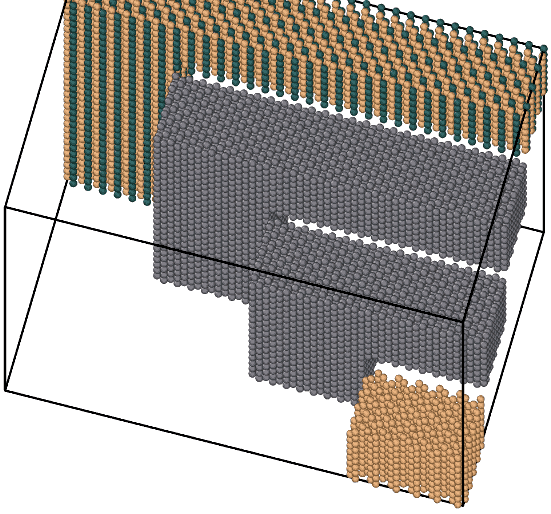
\includegraphics[width=1\textwidth]{images/lattice-full.png}
    \captionof{figure}{Simulation data saved with full lattice}
    \label{fig-save-lattice-full}
  \end{minipage}
  \qquad
  \begin{minipage}{.45\textwidth}
    \centering
    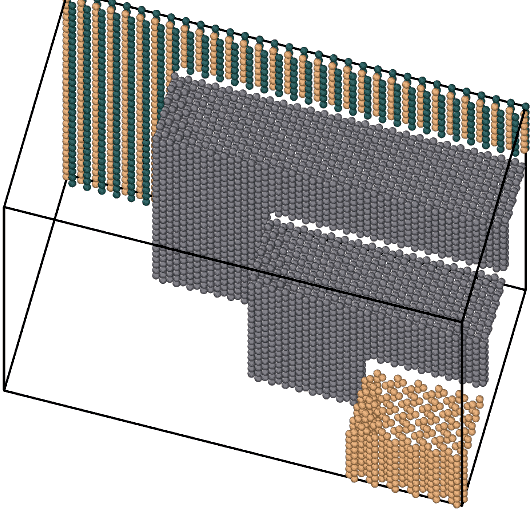
\includegraphics[width=1\textwidth]{images/lattice-near-gas.png}
    \captionof{figure}{Simulation data saved with lattice atoms near the solid-gas cell interface}
    \label{fig-save-lattice-near-gas}
  \end{minipage}
\end{figure}


\section{test}
\index{test}
Used mainly to test the code. It checks that some conditions are true, otherwise it aborts with an error.

\begin{description}

\item[array=$<$x1 y1 x2 y2 ... xn yn$>$] It requires the options \param{value=$<$value$>$}, \param{error=$<$error$>$}, \param{init=$<$init$>$} and \param{end=$<$end$>$} it checks that for all the xs between \param{init} and \param{end} the ys have a relative error smaller than \param{error} with respect to \param{value}. It prints the maximum relative error in the array. 
\item[array.2D] Similar to \param{array} but with input in 2D.
\item[array.3D] Similar to \param{array} but with input in 3D.
\item[arrays.2D] Compares that, given two 2D arrays in \param{one} and \param{two}, their $x$ and $y$ are identical and the values are withing a relative error smaller than \param{error}.
\item[float=$<$number$>$]  It requires the options \param{value=$<$value$>$} and \param{error=$<$error$>$}. It checks that \param{number} has a relative error smaller than \param{error} with respect to \param{value}. It prints the relative error in the array. 
\item[equal] It tests that \param{one} is equal to \param{two}.
\item[interval] Tests that \param{value} is between \param{begin} and \param{end}.
\item[not] Inverts the meaning of the test, i.e., returns OK it is NOT passed.
\item[tag=$<$tag$>$] Optional argument that allows setting a ``tag'' associated with this test. Useful to distinguish between test commands when many are called.
\end{description}

\subsection{Examples}
\begin{itemize}
\item \verb+test float=[extract count.particles] value=9 error=0+
\item \verb+test float=[extract count.particles particle=I] value=4 error=0+
\item \verb+test float=[extract count.particles particle=V] value=5 error=0+
\item \verb+test one="Hola" not equal two="hola"+
\end{itemize}


\chapter{Limitations}

\section{extract diffusivities}

Only tracks \idx{diffusivity} of impurities, i.e., not of I or V.

\chapter{Appendix}

\section{Binding energies}
\index{binding}

There is no {\tt Particle(binding) \{ pref\_b ener\_b \}}, instead there are two parameters: {\tt Dopant(formation) \{ pref\_d ener\_d \}} and {\tt Particle(formation) \{ pref\_p ener\_p \}}. Expressions for the variable change for energies and prefactors are shown below:
\begin{tabular}{lc}
  $pref_{Dop} = 1$ & $ener_{Dop} = 0$ \\
\end{tabular}

\begin{equation} 
  ener_{Part} = ener_{Dop} + ener_{IorV} - ener_{Bind}  
\end{equation}
\begin{equation}  
  pref_{Part} = \frac{pref_{Dop}}{pref_{Bind}} \cdot pref_{IorV} \cdot pref_{migIorV} \cdot v_{capt} 
\end{equation}

Where $ener_{IorV}$ is the \idx{formation energy} of interstitials or vacancies, $pref_{IorV}$ is the initial concentration of interstitials or vacancies, $pref_{migIorV}$ is the migration prefactor of interstitials or vacancies ({\tt IorV(migration)}), and $v_{capt}$ is the capture volume defined as:

\begin{equation}
  v_{capt} = 3.65 \cdot \lambda^3
\end{equation}

Where $\lambda$ is the \idx{migration jump}.

\subsection{Example}

\begin{itemize}
\item $E_f(C_i) = E_f(I) + E_f(C) - E_b(C_i)$
\item $\left.\frac{C_{C_i}}{C_{C_{ref}}}\right|_0 = \left.\frac{C_{C}}{C_{C_{ref}}}\right|_0 \cdot C_{I_0} \cdot \nu_{mI_0} \cdot v_{capt} \cdot \frac{1}{\nu{bin}(C_i)}$
\end{itemize}

\section{Copyrights}
\subsection{MMonCa}
For the \MMonCa\ code licensed under Apache 2:

\begin{verbatim}
Copyright 2011-2015 IMDEA Materials Institute, 
Getafe, Madrid, Spain
 
Licensed under the Apache License, Version 2.0 (the "License");
you may not use this file except in compliance with the License.
You may obtain a copy of the License at

   http://www.apache.org/licenses/LICENSE-2.0

Unless required by applicable law or agreed to in writing, software
distributed under the License is distributed on an "AS IS" BASIS,
WITHOUT WARRANTIES OR CONDITIONS OF ANY KIND, either express or implied.
See the License for the specific language governing permissions and
limitations under the License.
\end{verbatim}

\subsection{Random Number Generator}
The random number generator in \MMonCa\ is not distributed under Apache2, but under the following, different conditions:

\begin{verbatim}
   Copyright (C) 1997 - 2002, Makoto Matsumoto and Takuji Nishimura,
   All rights reserved.                          

   Redistribution and use in source and binary forms, with or without
   modification, are permitted provided that the following conditions
   are met:

     1. Redistributions of source code must retain the above copyright
        notice, this list of conditions and the following disclaimer.

     2. Redistributions in binary form must reproduce the above copyright
        notice, this list of conditions and the following disclaimer in the
        documentation and/or other materials provided with the distribution.

     3. The names of its contributors may not be used to endorse or promote 
        products derived from this software without specific prior written 
        permission.

   THIS SOFTWARE IS PROVIDED BY THE COPYRIGHT HOLDERS AND CONTRIBUTORS
   "AS IS" AND ANY EXPRESS OR IMPLIED WARRANTIES, INCLUDING, BUT NOT
   LIMITED TO, THE IMPLIED WARRANTIES OF MERCHANTABILITY AND FITNESS FOR
   A PARTICULAR PURPOSE ARE DISCLAIMED.  IN NO EVENT SHALL THE COPYRIGHT OWNER OR
   CONTRIBUTORS BE LIABLE FOR ANY DIRECT, INDIRECT, INCIDENTAL, SPECIAL,
   EXEMPLARY, OR CONSEQUENTIAL DAMAGES (INCLUDING, BUT NOT LIMITED TO,
   PROCUREMENT OF SUBSTITUTE GOODS OR SERVICES; LOSS OF USE, DATA, OR
   PROFITS; OR BUSINESS INTERRUPTION) HOWEVER CAUSED AND ON ANY THEORY OF
   LIABILITY, WHETHER IN CONTRACT, STRICT LIABILITY, OR TORT (INCLUDING
   NEGLIGENCE OR OTHERWISE) ARISING IN ANY WAY OUT OF THE USE OF THIS
   SOFTWARE, EVEN IF ADVISED OF THE POSSIBILITY OF SUCH DAMAGE.
\end{verbatim}



\bibliographystyle{apalike}
%\bibliographystyle{newapa}
\bibliography{articles}

\listoffigures
\listoftables
\printindex

\end{document}
